% multimodel-summary.tex -- multi-model summary of heat and cold burden under four
% climate scenarios, 2022-2050, written November 2026.
% Build: plain pdflatex (emacs, emacs-r container) or xelatex (bittensor-ubuntu), run
% twice. ozreport.cls, ozcolors.sty and ozfonts.sty in this directory are symlinks to
% ~/code/oz-templates/, and the logo is set by absolute path below, so no TEXINPUTS
% setting is needed.
% Tables in tex-tables/ and figures in figures/ are generated by
% output/report-multimodel-2026-11/ (run_pooling.sh, build_tables.R, country_extras.R,
% make_figures.R, make_report_tables.R). Do not edit them by hand.
\documentclass[11pt]{ozreport}
\usepackage{longtable}
\usepackage{lscape}
\usepackage{array}
\renewcommand{\ozdocmark}{/var/home/aoz/code/oz-templates/assets/ozlabs-seed-logo.pdf}
\newsavebox{\oztabbox}
% Full size if the table fits the text width, shrunk to fit if it does not.
\newcommand{\widetab}[1]{\begin{lrbox}{\oztabbox}\small\input{tex-tables/#1}\end{lrbox}\ifdim\wd\oztabbox>\textwidth\resizebox{\textwidth}{!}{\usebox{\oztabbox}}\else\usebox{\oztabbox}\fi}

\doctype{Working Report}
\shorttitle{Multi-Model Summary, 2022--2050}
\title{Heat and Cold Deaths Under Four Climate Scenarios, 2022--2050: A Multi-Model Summary}
\author{Aaron Osgood-Zimmerman \quad\textperiodcentered\quad OZ Labs, for the World Bank}
\date{November 6, 2026}

\begin{document}
\maketitle

\begin{abstract}
We ask how many deaths and years of life lost may be attributable to non-optimal temperatures between 2022 and 2050 under four climate scenarios, and how much of what can be said about those numbers survives disagreement between climate models and uncertainty in the underlying risk estimates. We applied the Global Burden of Disease exposure-response curves to daily temperature from 24 climate models in 204 countries, scaled each scenario to IHME's mortality forecasts, and pooled every combination of climate model and uncertainty draw (12,000 values per number) into one interval. Under SSP2-4.5, world heat deaths rise from 431,244 per year in 2022--2030 (95\% interval 328,460 to 570,407) to 729,507 in 2041--2050 (499,064 to 1,074,365), and cold deaths from 1,483,673 (1,302,682 to 1,661,329) to 1,998,935 (1,602,802 to 2,423,909). Most of this rise occurs in every scenario: by 2041--2050, SSP5-8.5 has 1.127 times the heat deaths of SSP2-4.5 and 0.976 times the cold deaths, and the two nearly offset, so that total temperature-attributable deaths differ by a ratio of 1.016 with an interval on the difference that includes zero. These numbers rest on IHME's forecasts of population and mortality and on curves that do not change over time, and they are not forecasts of what will happen; they do not test adaptation, and the intervals do not include every source of uncertainty.
\end{abstract}

\section{Introduction}

The World Bank's Global Climate-Health Program wishes to know what future cause-specific mortality attributable to temperature could look like under different climate scenarios, holding non-temperature risks at their forecast values. Our aim here is to summarize the finished scenario runs in the form agreed at the team meeting of October 27, 2026: one number and one set of uncertainty intervals for each quantity, built on a common set of climate models, showing heat, cold and their sum side by side, with breakdowns by cause, age and sex, and income group, as averages over decades rather than single years.

The rest of this report is organized as follows. Section~\ref{sec:methods} describes how the numbers are constructed. Section~\ref{sec:results} gives the results: world totals, the differences between scenarios, where the uncertainty comes from, income groups, countries (including two that we mark with an asterisk), causes, age and sex, years of life lost, the year heat overtakes cold, and the sensitivity to the choice of climate models. Section~\ref{sec:checks} says how the numbers were checked, and Section~\ref{sec:discussion} sets out what we would not claim from them. Country tables are in the appendices.

\clearpage
\section{Data and methods}\label{sec:methods}

\subsection{Attributable deaths}

We follow the approach of Burkart et al.\ (Lancet, 2021) and the Global Burden of Disease (GBD) study. For each location, 17 causes of death are linked to temperature through cause-specific exposure-response curves, which give the relative risk of death at a given daily temperature within a temperature zone defined by a pixel's annual mean temperature. A pixel's zone is reassigned each year from that year's mean, but the curves themselves do not change over time. Each cause-specific population attributable fraction (PAF), the share of that cause's deaths attributed to temperature, is computed against a theoretical minimum risk exposure level (TMREL), the temperature of lowest death-weighted risk, which we derive separately for each uncertainty draw and year from that draw's curves and cause-of-death mix. Pixel-level results are weighted by population to the national level. We use 500 uncertainty draws, and the same draw index $d$ refers to the same draw of the curves and of the mortality forecast across years, countries, scenarios and climate models, which is what allows the differences below to be taken draw by draw.

Daily temperature comes from the World Bank Climate Change Knowledge Portal's downscaled and bias-corrected CMIP6 product at 0.25 degrees. We use four Shared Socioeconomic Pathway (SSP) scenarios, SSP1-2.6, SSP2-4.5, SSP3-7.0 and SSP5-8.5, for 2022--2050. Deaths come from IHME's GBD 2021 Foresight reference forecast, which IHME defines under SSP2-4.5.

\subsection{Scaling to IHME's forecasts}

Because IHME's mortality forecast already embeds SSP2-4.5 temperature, deaths under another scenario are obtained by removing that temperature component and applying the scenario's own (the step we have called Workflow B, which is the approach set out in the World Bank's data request to IHME). For cause $c$ and draw $d$, with $m$ the IHME forecast deaths and $\mathrm{PAF}$ the non-optimal attributable fraction,
\begin{equation*}
  m^{\mathrm{scaled}}_{c,d} = m_{c,d} \times \frac{S^{\mathrm{target}}_{c,d}}{S^{\mathrm{SSP2\text{-}4.5}}_{c,d}},
  \qquad S = \frac{1}{1 - \mathrm{PAF}},
\end{equation*}
for the 13 causes in which IHME's forecast carries a temperature scalar; for the remaining four (cardiomyopathy and myocarditis, animal contact, forces of nature, and other unintentional injuries) the ratio is set to 1. Attributable deaths are then $m^{\mathrm{scaled}}$ times the scenario's PAF. SSP2-4.5 scaled against itself reproduces the unscaled burden, and the team chose to keep this step for the headline numbers; at world level it moves totals by less than 0.15\%, so it matters little for what follows.

\subsection{Pooling across climate models}

Each number in this report is computed from 12,000 values, the 24 climate models run under all four scenarios crossed with 500 draws. An interval is taken from the quantiles of that pool, so disagreement between climate models is part of it, and each model carries equal weight. Reported intervals are 95\% (the GBD convention), 80\%, and 66\% (the IPCC's ``likely'' range). Sums over locations or years are taken within a draw and model before pooling, and a difference between scenarios is taken draw by draw within a model before pooling, so that the uncertainty shared by the two scenarios does not enter the difference. Decades are 2022--2030 (nine years), 2031--2040 and 2041--2050, and every value is per year.

The 24 models are not 24 independent results: several share code and history (two EC-Earth, two MPI, two NorESM, two INM, two CNRM, two MIROC, and the HadGEM and UKESM family). Pooled intervals treat the models as a sample, and we would not read them as probabilities in any strict sense.

\subsection{Measures}

Rates are crude deaths per 100,000 people per year, with population taken from the mean of IHME's forecast draws for the slice in question, averaged over the decade's years; because population is held at that mean, a rate's interval reflects the deaths only. Crude rates are not age-standardized, so a rise can reflect an older population and not only a higher risk at each age. Years of life lost (YLLs) use our national definition, deaths times the country's UN World Population Prospects remaining life expectancy at the start of the 5-year age group (80+ uses age 80). These are not comparable with GBD's YLLs, which use a reference life table. Income groups are the World Bank's, from its country list as downloaded on November 6, 2026, applied to all years: 71 high income, 58 upper middle, 47 lower middle and 25 low income. Taiwan is absent from that list and is taken as high income from the Bank's classification spreadsheet, and Cook Islands, Niue and Tokelau appear in neither and stay unclassified (they sum to about one death per year). This mapping has not yet been reviewed by a second person.

\section{Results}\label{sec:results}

\subsection{How many deaths, and how do they change over time?}

Table~\ref{tab:world} gives world totals for each scenario and decade, and Figure~\ref{fig:decades} shows the same numbers with the three interval levels. Under SSP2-4.5, heat deaths rise by 69\% between 2022--2030 and 2041--2050 and cold deaths by 35\%, and heat's share of the two together rises from 22.5\% to 26.7\%, so cold remains the larger burden throughout the period in every scenario. As a rate, heat deaths go from 5.25 to 7.89 per 100,000 people per year and cold from 18.06 to 21.63, smaller increases than in counts because population grows from 8.22 to 9.24 billion.

\begin{table}[htbp]
\centering
\caption{World deaths per year attributable to heat and cold, 24 common climate models, by scenario and decade: pooled mean and 95\% interval.}\label{tab:world}
\widetab{tab_world.tex}
\end{table}

\begin{figure}[htbp]
\centering
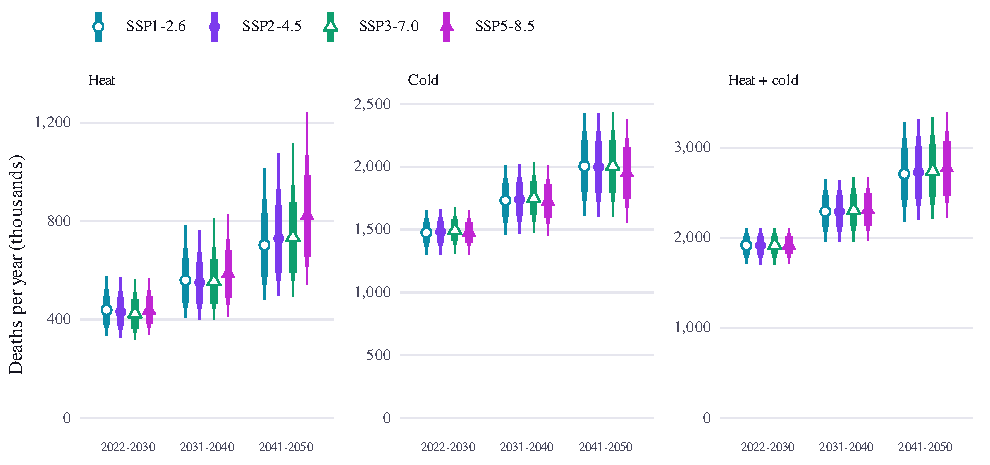
\includegraphics[width=\textwidth]{figures/fig_world_decades.pdf}
\caption{World deaths per year by decade and scenario, 24 common climate models. The point is the pooled mean; the thin, medium and thick bars are the 95\%, 80\% and 66\% intervals. The vertical scales differ between panels.}\label{fig:decades}
\end{figure}

Why do cold deaths rise when the world is warming? The rise follows IHME's forecast of deaths from these 17 causes, which grows from 32.0 to 43.4 million per year between the two decades. Cold's share of those deaths stays nearly flat (4.66\% to 4.62\%), while heat's rises (1.32\% to 1.69\%). This is consistent with an aging population moving into the causes and ages most affected by cold, at about the rate that warming reduces cold exposure, but we have not split this further. An earlier split of the rise in heat deaths, on single years under SSP2-4.5 (2022 to 2050, as model means, without uncertainty; \texttt{docs/reviews/heat-rise-decomposition-2026-10-27.org}), attributes the $+106$\% to population size ($+23$ percentage points), aging ($+106$), lower death rates ($-70$) and a higher heat share ($+47$), which suggests that most of the rise in heat deaths would occur without further warming, as far as that split reaches.

Figure~\ref{fig:yearly} shows the same series by year. It is shown to make clear why we do not report single years: world heat deaths within one model change by $-19$\% to $+29$\% from one year to the next (1st to 99th percentile over runs), and by as much as $+47$\% in one case (MIROC-ES2L under SSP3-7.0 in 2032, of which India accounts for 77,100 of the 176,124 added deaths). Such spikes are not shared across models, which is consistent with simulated weather and not with an error in a common input.

\begin{figure}[htbp]
\centering
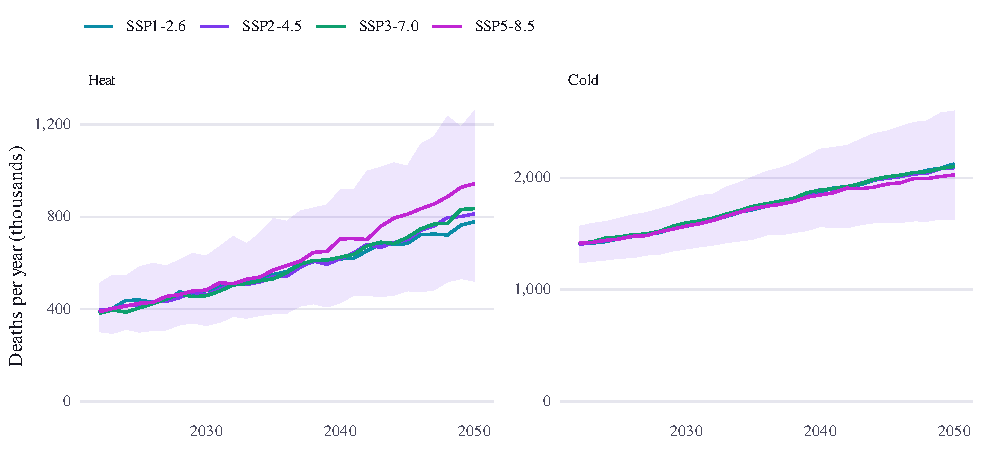
\includegraphics[width=\textwidth]{figures/fig_world_yearly.pdf}
\caption{World deaths per year by single year: mean over the 24 common climate models and 500 draws, for each scenario. The shaded band is the pooled 95\% interval for SSP2-4.5. Single years are shown only to illustrate variability; we report decades.}\label{fig:yearly}
\end{figure}

\subsection{How much do the scenarios differ?}

Table~\ref{tab:diff} and Figure~\ref{fig:diff} set each scenario against SSP2-4.5. The clearest departure is SSP5-8.5 in 2041--2050, with 92,442 more heat deaths per year (95\% interval 24,344 to 206,886; ratio 1.127, and higher than SSP2-4.5 in all 24 models) and 48,176 fewer cold deaths ($-106{,}725$ to $-16{,}804$; ratio 0.976, lower in all 24). Because these offset, the total differs by 44,266 ($-14{,}239$ to $141{,}455$; ratio 1.016), and 21 of 24 models have a higher total. For SSP1-2.6 in the same decade, heat is lower by 26,357 ($-106{,}815$ to $36{,}835$; ratio 0.964, with 7 of 24 models above SSP2-4.5), an interval which includes zero. SSP3-7.0 cannot be told apart from SSP2-4.5 by this measure (heat ratio 1.008, 13 of 24 models above).

\begin{table}[htbp]
\centering
\caption{Target scenario against SSP2-4.5, world deaths per year, 24 common models. Ratio is target mean over SSP2-4.5 mean. Difference is taken draw by draw within a model and then pooled: mean and 95\% interval.}\label{tab:diff}
\widetab{tab_diff.tex}
\end{table}

\begin{figure}[htbp]
\centering
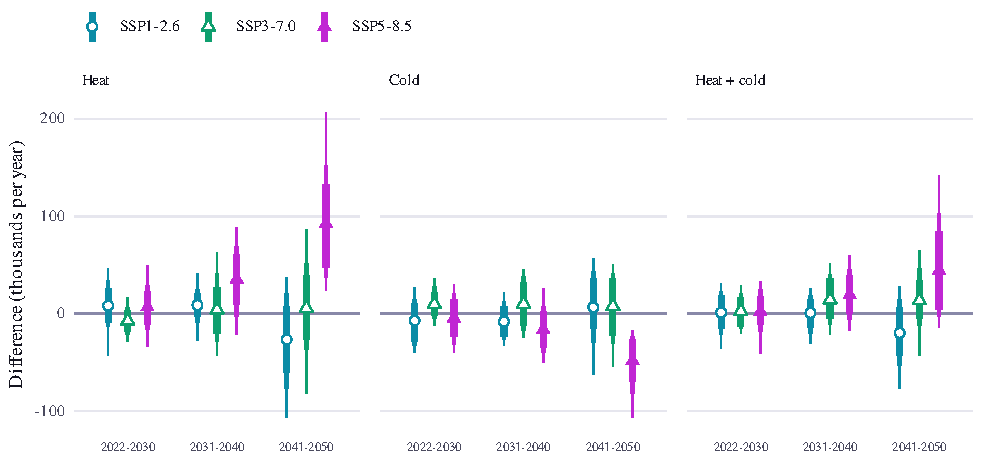
\includegraphics[width=\textwidth]{figures/fig_world_diff.pdf}
\caption{Difference from SSP2-4.5 in world deaths per year, by decade, with the 95\%, 80\% and 66\% intervals (thin, medium, thick bars) of the draw-by-draw difference, 24 common climate models.}\label{fig:diff}
\end{figure}

Before 2040 the order is not the one a reader might expect: SSP1-2.6 has slightly more heat deaths than SSP2-4.5 (ratios 1.019 and 1.016, with 17 and 19 of 24 models above) and SSP3-7.0 slightly fewer in 2022--2030 (0.983, 7 of 24). Temperature is consistent with this: in a death-weighted average over countries, SSP1-2.6 is 0.11\textdegree{}C warmer than SSP2-4.5 in 2030 and 0.25\textdegree{}C cooler by 2050 (from the four years we hold temperature for; review of October 26, 2026). One possibility is the faster reduction of cooling aerosols under SSP1-2.6, which we have not tested.

At country level the same picture holds with less power. The 95\% interval for the SSP5-8.5 heat difference in 2041--2050 is entirely above zero in 39 of 204 countries and entirely below in none. For SSP1-2.6 it is entirely below zero in one country and for SSP3-7.0 in none. With 204 comparisons, some intervals would exclude zero even with no underlying difference, so these counts are not rates, and the differences between countries should not be overread.

\subsection{Where does the uncertainty come from?}

For world heat deaths, about half of the pooled variance is between climate models (0.41 to 0.57, by scenario and decade), and the remainder comes from the draws of the curves and the mortality forecast. For cold, the share between models is about a tenth (0.07 to 0.14). For heat plus cold it is only 0.02 to 0.04, because a model that runs warm has more heat deaths and fewer cold deaths. The sum is thus much less sensitive to the choice of climate model than either part, and its interval (coefficient of variation about 0.11 in 2041--2050) is carried almost entirely by the exposure-response curves and the mortality forecast. Table~\ref{tab:levels} gives the three interval levels and the range of the 24 model means for the most-compared cells.

\begin{table}[htbp]
\centering
\caption{World deaths per year, 2041--2050, 24 common models: pooled mean, 95\%, 80\% and 66\% intervals, and the lowest and highest of the 24 model means.}\label{tab:levels}
\widetab{tab_levels.tex}
\end{table}

\subsection{How do income groups differ?}

Table~\ref{tab:income} and Figure~\ref{fig:income} give the income groups. The burden differs in kind. Cold rates under SSP2-4.5 in 2041--2050 are high in the high-income (40.2 per 100,000 per year) and upper-middle-income (35.1) groups and low in the lower-middle (7.5) and low-income (5.4) groups, while heat rates are highest in the lower-middle-income group (10.7), compared with 7.4, 5.2 and 4.1 in the upper-middle, low and high-income groups. These are crude rates, and much of the contrast in cold is likely age structure: high-income countries are older, and most cold deaths occur at 65 and above. Low- and middle-income countries hold 92\% of world heat deaths in that decade and 71\% of cold deaths. The proportional effect of SSP5-8.5 on heat is similar across the wider groups (1.109 in high-income and 1.128 in low- and middle-income countries), but the difference in deaths is not: 6,446 and 85,995 per year.

\begin{table}[htbp]
\centering
\caption{Deaths per year and crude rate per 100,000 per year (95\% interval), by World Bank income group, SSP2-4.5, 2041--2050, 24 common models, and the SSP5-8.5 to SSP2-4.5 ratio of means. World equals the four income groups plus three unclassified locations.}\label{tab:income}
\widetab{tab_income.tex}
\end{table}

\begin{figure}[htbp]
\centering
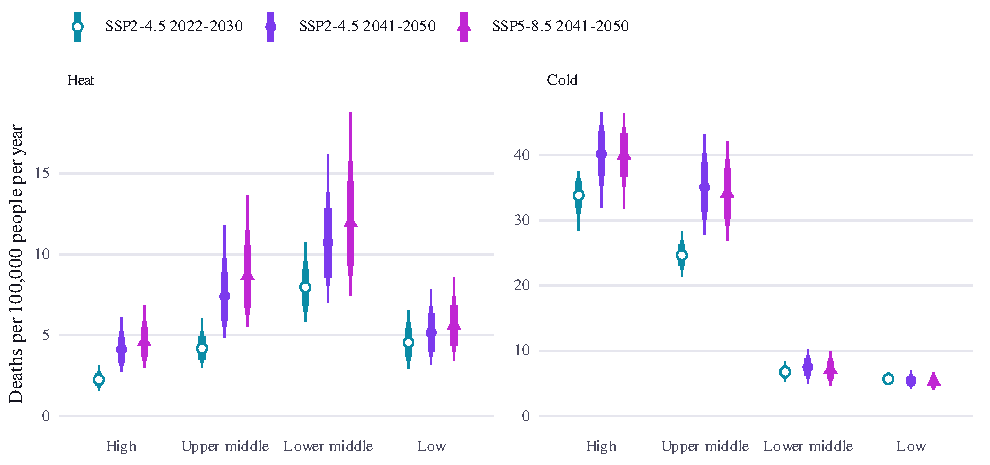
\includegraphics[width=\textwidth]{figures/fig_income_rates.pdf}
\caption{Crude deaths per 100,000 people per year by World Bank income group, 24 common climate models: SSP2-4.5 in 2022--2030 and 2041--2050, and SSP5-8.5 in 2041--2050. The point is the pooled mean; thin, medium and thick bars are the 95\%, 80\% and 66\% intervals. The vertical scales differ between panels.}\label{fig:income}
\end{figure}

\subsection{Which countries, and which need a caution?}

The world totals are concentrated. In 2041--2050 under SSP2-4.5, India accounts for 31.7\% of heat deaths (231,555 per year, 95\% interval 146,386 to 359,901) and China for 39.6\% of cold deaths (792,478, from 621,344 to 978,559), and the five largest countries hold 58.6\% of heat deaths and 58.0\% of cold deaths. Figure~\ref{fig:maps} maps the rates, and Table~\ref{tab:country} in Appendix~\ref{app:country} lists every country.

\begin{figure}[htbp]
\centering
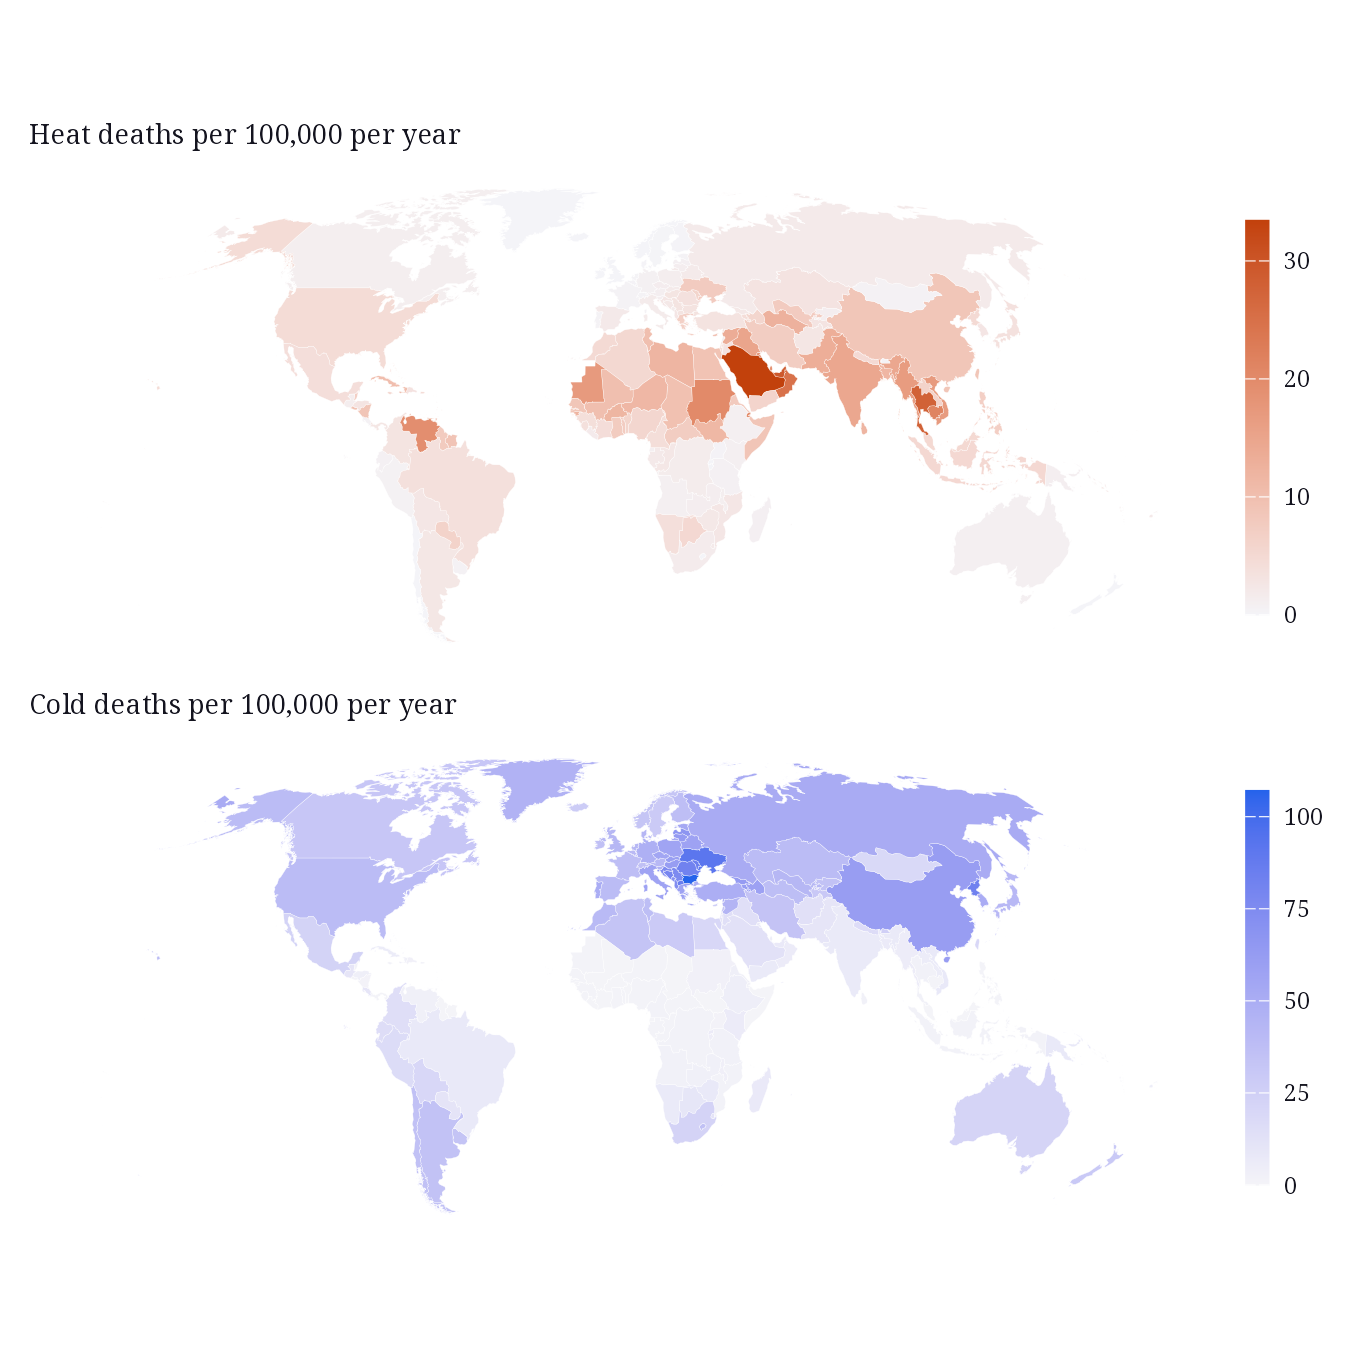
\includegraphics[width=0.92\textwidth]{figures/fig_maps.png}
\caption{Crude heat and cold deaths per 100,000 people per year, by country, SSP2-4.5, 2041--2050, pooled mean over the 24 common climate models. Each panel has its own scale. The maps do not show uncertainty, and small island states are barely visible; see Table~\ref{tab:country}.}\label{fig:maps}
\end{figure}

Two cautions apply to reading the country numbers. The first concerns the Gulf states, which lead the heat rate table: Saudi Arabia 33.4 per 100,000 per year (18.6 to 54.1), United Arab Emirates 29.2 (14.5 to 47.6). IHME's forecast multiplies 17-cause deaths in the United Arab Emirates by 10.6 between 2022 and 2050 (10,961 to 116,058), as well as by 8.2 in Qatar, 4.3 in Oman, 4.1 in Bahrain and Kuwait, and 3.2 in Saudi Arabia, against 1.52 for the world, and its population aged 65 and over in the United Arab Emirates goes from 198,137 to 4,717,387. This is consistent with migrant workers being forecast to age in place, which is our guess and not something the files state. The pipeline follows these inputs as given, so the Gulf rates in 2041--2050 depend on that forecast.

The second concerns disasters. IHME's forecast draws for the cause ``exposure to forces of nature'' include, in a few draws, deaths on the scale of a major event. A PAF of a percent or two on those deaths swings a small country's total, and in Haiti such draws also pull the derived TMREL to the bottom of its search range, which then applies to all 17 causes in that draw (review of September 14, 2026). We keep all 17 causes in every headline number, as the team decided, and mark the two countries where this matters most, Haiti and Honduras, with an asterisk, showing the totals beside the same totals without that cause (Table~\ref{tab:asterisk}). The column without the cause removes only that cause's own deaths and not its effect on the TMRELs, so it does not undo the second mechanism in Haiti, and it should not be read as a corrected estimate: Haiti's interval without the cause includes zero, which we suspect is for that reason. For Haiti, the mean is a poor summary of the distribution; the median non-optimal value in a single year is 539 deaths where the highest is 115,656. Across all countries under SSP2-4.5 in 2041--2050, the upper bound of the 95\% interval moves by more than 2\% in 8 of 204 and by more than 10\% only in these two. The effect on larger aggregates is small: in 2041--2050, 645,009 against 642,870 deaths per year for the lower-middle-income group, in which both countries fall, and 2,728,442 against 2,727,440 for the world. Single draws show the same feature elsewhere (19,041 deaths in one year of one draw in Puerto Rico, against a median of 129; 81,968 in Myanmar, against 11,516), which is a further reason to avoid single-year country values, although in these cases decade means and intervals are little affected.

\begin{table}[htbp]
\centering
\caption{The two countries marked with an asterisk: heat plus cold deaths per year under SSP2-4.5, 24 common models, mean and 95\% interval, with all 17 causes (the headline number) and without the cause ``exposure to forces of nature''.}\label{tab:asterisk}
\widetab{tab_asterisk.tex}
\end{table}

\subsection{Which causes?}

Table~\ref{tab:cause} and Figure~\ref{fig:causes} give the causes for 2041--2050 under SSP2-4.5. Ischemic heart disease and stroke are the largest for heat (168,892 and 144,203 deaths per year, together 43\% of the total), followed by diabetes, chronic obstructive pulmonary disease (COPD) and lower respiratory infections. For cold, ischemic heart disease leads (562,182), followed by COPD (475,014) and stroke (413,001). Diabetes is unusual in having about equal heat and cold deaths (85,485 and 84,124). The nine injury causes add 104,988 heat deaths per year, and all nine have negative mean cold values, summing to $-118{,}825$: the curves indicate lower injury risk on cold days than at the TMREL. These negative values stay in the cold total, so a reader adding only the positive causes will arrive at a larger number than ours.

\begin{table}[htbp]
\centering
\caption{Deaths per year by cause, SSP2-4.5, 2041--2050, 24 common models: world mean with 95\% interval, and means for the high-income group and the low- and middle-income (LMIC) group.}\label{tab:cause}
\widetab{tab_cause.tex}
\end{table}

\begin{figure}[htbp]
\centering
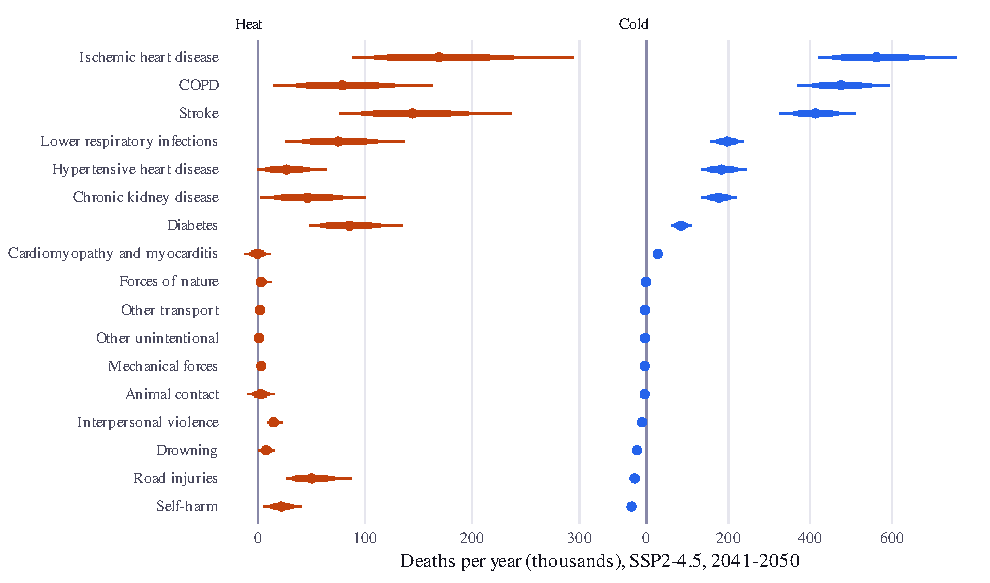
\includegraphics[width=\textwidth]{figures/fig_causes.pdf}
\caption{World deaths per year by cause, SSP2-4.5, 2041--2050, 24 common climate models. Thin, medium and thick bars are the 95\%, 80\% and 66\% intervals. The horizontal scales differ between panels, and causes are ordered by mean cold deaths.}\label{fig:causes}
\end{figure}

Breakdowns by cause become much less certain as they get narrower. At world level under SSP2-4.5, the 95\% interval includes zero for 7 of 17 causes for heat and 1 of 17 for cold. For a single cause in a single country, it includes zero in most cells for heat and about a third of cells for cold (60.2\% and 30.7\% of 3,452 non-zero cells under SSP5-8.5). For that reason we report causes at world and income-group level here, and country by cause only in Appendix~\ref{app:cause}, where cells whose interval includes zero are in parentheses. Plain country totals rarely have this problem: for deaths, the interval includes zero in at most 2 of 204 countries.

\subsection{Which ages, and which sex?}

Table~\ref{tab:age} and Figure~\ref{fig:age} show the three age groups the team asked for. People aged 65 and over account for a growing majority of attributable deaths: 59\% of heat deaths in 2022--2030 and 72\% in 2041--2050, and 88\% and 93\% of cold deaths. Children under 5 account for 4.9\% of heat deaths in 2022--2030 and 1.5\% in 2041--2050, falling in count as well (21,009 to 10,766 per year) with falling under-5 mortality in the forecast. Women aged 15 to 49 have 18,679 and 19,106 heat deaths per year in the two decades. Heat deaths at 15 to 49 are about three times higher in men than in women, which we suspect reflects the injury causes, although we have not split these slices by cause. For the same reason, we suspect, men aged 15 to 49 have a negative cold total at world level ($-7{,}116$ deaths per year in 2041--2050, with an interval from $-13{,}182$ to $-725$).

\begin{table}[htbp]
\centering
\caption{World deaths per year and crude rate per 100,000 in that age and sex group, SSP2-4.5, 24 common models, mean and 95\% interval. The slices do not sum to the total: ages 5--14 and 50--64 are not exported.}\label{tab:age}
\widetab{tab_age.tex}
\end{table}

\begin{figure}[htbp]
\centering
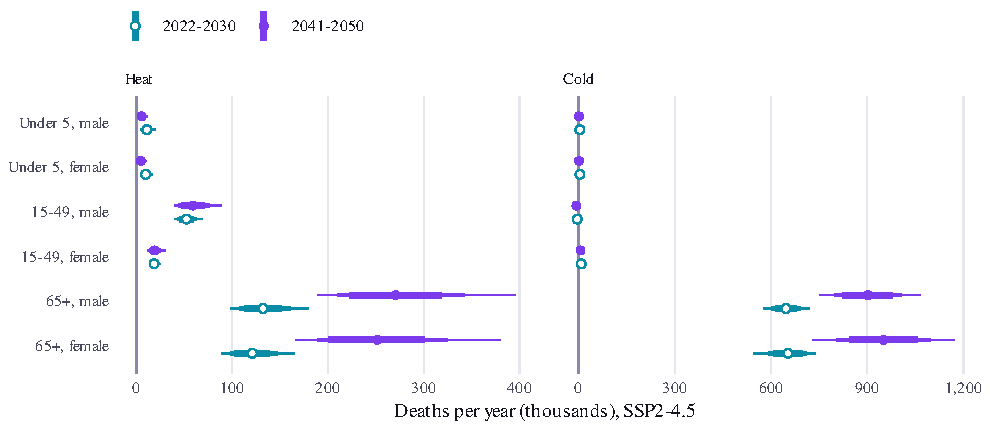
\includegraphics[width=\textwidth]{figures/fig_age.pdf}
\caption{World deaths per year by age group and sex, SSP2-4.5, 2022--2030 and 2041--2050, 24 common climate models. Thin, medium and thick bars are the 95\%, 80\% and 66\% intervals. The horizontal scales differ between panels.}\label{fig:age}
\end{figure}

\subsection{What about years of life lost?}

Under SSP2-4.5, heat accounts for 12.8 million YLLs per year in 2041--2050 (95\% interval 8.7 to 18.9 million) and cold for 23.8 million (18.9 to 29.4 million). Heat is a larger share of YLLs than of deaths (35\% against 27\%) because heat deaths include more young people. The ratio of SSP5-8.5 to SSP2-4.5 is 1.119 for heat YLLs and 0.976 for cold YLLs.

One feature needs care in any table of country YLLs. Because injury causes have negative cold values and fall at young ages, where remaining life expectancy is high, a country's cold YLLs can be negative alongside positive cold deaths: 21 countries in 2022--2030, 13 in 2031--2040 and 8 in 2041--2050 under SSP2-4.5, with the interval including zero in 69, 60 and 54. For example, in Burkina Faso under SSP1-2.6 in 2041--2050, cold deaths are $+114.6$ per year and cold YLLs $-294.9$. It follows that YLLs per death is not a usable statistic wherever signs mix (it reads 110.7 for men aged 15 to 49 at world level in 2022--2030). Where signs do not mix it behaves as expected: about 10 to 12 years at 65 and over, about 41 to 45 for heat at 15 to 49, and about 63 to 70 for heat under 5.

\subsection{When does heat overtake cold?}

Samuel asked for the year in which heat deaths overtake cold deaths in each country. To answer this we fitted, for each combination of climate model, draw and scenario, a straight line to yearly heat minus cold over 2022--2050, and took the crossing as the year in which the line reaches zero, recording ``before 2022'' if it is already above zero in 2022 and ``after 2050'' if it is still below zero in 2050. Table~\ref{tab:crosscount} counts countries by where the median of those 12,000 crossings falls, and this replaces our earlier first look, which used only model means. A straight line is a strong simplification, and we offer these as a summary of direction and not as estimates of a date.

\begin{table}[htbp]
\centering
\caption{Countries (of 204) by where the median year heat overtakes cold falls, over 12,000 (model, draw) pairs, 24 common models.}\label{tab:crosscount}
{\small\begin{tabular}{lcccc}
\toprule
Where the median falls & SSP1-2.6 & SSP2-4.5 & SSP3-7.0 & SSP5-8.5 \\
\midrule
Heat above cold already in 2022 & 83 & 82 & 80 & 75 \\
Median crossing within 2022--2050 & 6 & 8 & 11 & 16 \\
Heat stays below cold through 2050 & 115 & 114 & 113 & 113 \\
\bottomrule
\end{tabular}
}
\end{table}

In most countries the answer is settled at one end. Heat is above cold from the start in India (in 85\% of pairs) and Nigeria (100\%), and stays below it through 2050 in China, the United States and the Russian Federation (100\%). The year itself, however, cannot be pinned down in the countries where it falls within the period: under SSP2-4.5 there are eight (Table~\ref{tab:crosslist}), and in all eight the 95\% interval for the year runs from before 2022 to after 2050. We would therefore report for those countries the share of pairs in each category and not a year. Warming moves countries in the expected direction, with 16 countries in the middle category under SSP5-8.5, against 6 under SSP1-2.6, though the numbers are small.

\begin{table}[htbp]
\centering
\caption{Countries whose median crossing falls within 2022--2050 under SSP2-4.5: median year and the share of (model, draw) pairs in each category.}\label{tab:crosslist}
{\small\begin{tabular}{lcccc}
\toprule
Country & Median year & Before 2022 & Within 2022--2050 & After 2050 \\
\midrule
Tonga & 2023 & 48\% & 40\% & 12\% \\
Sao Tome and Principe & 2027 & 37\% & 41\% & 23\% \\
Iraq & 2033 & 33\% & 36\% & 32\% \\
Dominican Republic & 2034 & 23\% & 46\% & 32\% \\
Vanuatu & 2036 & 16\% & 51\% & 33\% \\
Lao People's Democratic Republic & 2039 & 20\% & 45\% & 36\% \\
Honduras & 2040 & 30\% & 27\% & 43\% \\
Niue & 2042 & 12\% & 49\% & 39\% \\
\bottomrule
\end{tabular}
}
\end{table}

\subsection{Do the results depend on which climate models are used?}

The headline numbers use the 24 models common to all four scenarios. Table~\ref{tab:sensitivity} compares two alternatives: paired sets, in which each target uses every model that has both its run and an SSP2-4.5 run (26, 24 and 27 models), and all available, in which the target uses its models and SSP2-4.5 uses all 27. The ratio moves by up to 0.7 points for heat under SSP5-8.5 (1.127, 1.134 and 1.134) and by a point for SSP3-7.0 under the all-available set (0.998 against 1.008), in which different models are being compared, and the conclusions above do not change. Models with no SSP2-4.5 run cannot be scaled and so are absent from all three sets; among them are HadGEM3-GC31-MM and TaiESM1, two of the three hottest of the 29 models under SSP5-8.5 in 2041--2050.

\begin{table}[htbp]
\centering
\caption{World mean deaths per year for the target scenario, and ratio to SSP2-4.5, 2041--2050, under the three choices of climate models.}\label{tab:sensitivity}
\widetab{tab_sensitivity.tex}
\end{table}

\section{How the numbers were checked}\label{sec:checks}

The per-draw files were compared with the summary tables Caspar's machine produced independently of them. For all 204 countries, the yearly means and quantiles match those tables to within the 6-digit rounding of the export, causes summed in a draw match the yearly totals, the 17 causes and three age groups are complete in every file, and under-5 YLLs per death lie within the life table's value for the right sex, apart from a small number of rows (90 of 162,344) that we attribute to deaths of mixed sign. Pooled numbers were then computed twice, by the production script and by independent code, and these agree to within $10^{-10}$ in relative terms at world level and for all 253,368 country-by-cause and country-by-age cells of the three target scenarios. Before pooling we wrote down what we expected, and the world heat values matched to within 1 death in 1,000. Two expectations were wrong: we expected cold deaths to be about flat (they rise by 35\%), and we expected stroke to rank second for cold (it is COPD). The full review is in \texttt{docs/reviews/workflow-b-draw-export-review-2026-11-05.org}. Against GBD 2023-round estimates for 2022, our earlier comparison on the SSP2-4.5 runs gave ratios of 0.68 to 0.77 for heat and 0.93 to 0.98 for cold (review of September 24, 2026), so our heat numbers run below that reference, and we have not resolved why.

\section{Discussion}\label{sec:discussion}

The main reading of these results is that most of the rise in temperature-attributable deaths to 2050 is common to all four scenarios, and that the scenarios differ, by 2041--2050, in the split between heat and cold more than in the total. That reading rests on scenarios whose temperatures have not diverged far by 2050 (SSP5-8.5 is 0.50\textdegree{}C warmer than SSP2-4.5 in 2050 in a death-weighted average over countries, from the review of October 26, 2026), and we would not extend it beyond 2050, when the scenarios diverge further.

Several assumptions limit what these numbers can say. First, the exposure-response curves do not change over time, so nothing here tests adaptation, whether through air conditioning, health systems or physiology. Second, we hold IHME's population and mortality forecasts fixed across scenarios, apart from the temperature scalar, so climate does not affect the other risks, and the forecasts' own features (the Gulf states, or event-scale disaster draws) pass straight through. Third, the intervals cover the curves, the mortality forecast's draws and disagreement between climate models, on 24 models that are not independent; they do not cover structural choices such as the bias correction of the temperature inputs, the 0.25-degree resolution, or the choice of curves. Fourth, our YLLs are not GBD's, and our rates are crude.

Open items remain. The SSP3-7.0 result in parts of Western and Central Europe (fewer heat deaths with annual mean temperature about unchanged) has not been explained, and would need summer temperature from Caspar's machine. A split of the rise by decade would also need age-by-year output from that machine. The income-group mapping needs a check by a second person, and the Foresight forecast's handling of migrant populations is something we would want to ask IHME about before leaning on the Gulf rates.

\appendix

\section{Country totals}\label{app:country}

Table~\ref{tab:country} lists every country under SSP2-4.5 for 2041--2050. The other scenarios, decades, measures and interval levels are in \texttt{tables/country\_totals.csv} alongside this report. Ratios mean little where the deaths are few: Greenland's 3.01 rests on far below one heat death per year, so the deaths should be read beside every ratio.

{\scriptsize\setlength{\tabcolsep}{3pt}
\begin{longtable}{lccrcrrr}
\caption{Country totals under SSP2-4.5, 2041--2050, on the 24 common models: mean deaths per year with 95\% interval, crude rate per 100,000 people per year, and the SSP5-8.5 to SSP2-4.5 ratio of mean heat deaths. Income group: H high, UM upper middle, LM lower middle, L low, -- not classified. An asterisk marks the two countries whose totals carry a disaster-forecast tail.}\label{tab:country}\\
\toprule
Country & Inc. & Heat deaths (95\%) & Rate & Cold deaths (95\%) & Rate & Net rate & Ratio \\
\midrule
\endfirsthead
\toprule
Country & Inc. & Heat deaths (95\%) & Rate & Cold deaths (95\%) & Rate & Net rate & Ratio \\
\midrule
\endhead
\bottomrule
\endfoot
Afghanistan & L & 1,704 (967 to 2,761) & 2.7 & 8,718 (5,281 to 13,473) & 13.9 & 16.6 & 1.09 \\
Albania & UM & 62 (20 to 134) & 2.6 & 1,761 (1,358 to 2,210) & 73.4 & 76.0 & 1.42 \\
Algeria & UM & 2,895 (1,642 to 4,755) & 5.3 & 18,112 (13,192 to 24,417) & 33.3 & 38.6 & 1.19 \\
American Samoa & H & 2.9 (0.9 to 6.3) & 4.8 & 0.1 (0.0 to 0.5) & 0.2 & 5.0 & 1.23 \\
Andorra & H & 0.0 (0.0 to 0.1) & 0.0 & 37 (26 to 50) & 48.7 & 48.7 & 1.85 \\
Angola & LM & 554 (236 to 1,089) & 0.9 & 1,278 (788 to 1,803) & 2.1 & 2.9 & 1.25 \\
Antigua and Barbuda & H & 3.5 (0.8 to 7.8) & 3.8 & 0.7 (0.1 to 2.1) & 0.8 & 4.6 & 1.27 \\
Argentina & UM & 1,203 (659 to 1,929) & 2.5 & 16,752 (13,271 to 20,832) & 35.1 & 37.6 & 1.21 \\
Armenia & UM & 106 (42 to 216) & 4.3 & 1,529 (1,130 to 2,010) & 61.8 & 66.1 & 1.13 \\
Australia & H & 298 (169 to 487) & 0.9 & 7,412 (5,709 to 9,145) & 21.9 & 22.8 & 1.17 \\
Austria & H & 104 (38 to 219) & 1.1 & 4,110 (3,178 to 4,988) & 41.8 & 42.8 & 1.15 \\
Azerbaijan & UM & 640 (328 to 1,087) & 5.6 & 6,660 (4,844 to 9,002) & 58.5 & 64.1 & 1.21 \\
Bahamas & H & 21 (8.2 to 41) & 4.8 & 18 (7.0 to 31) & 4.1 & 9.0 & 1.24 \\
Bahrain & H & 548 (285 to 902) & 25.7 & 190 (72 to 315) & 8.9 & 34.6 & 1.10 \\
Bangladesh & LM & 20,979 (10,195 to 35,270) & 11.6 & 12,214 (6,759 to 19,001) & 6.8 & 18.4 & 1.18 \\
Barbados & H & 13 (3.6 to 28) & 4.8 & 0.9 (0.0 to 3.2) & 0.3 & 5.1 & 1.27 \\
Belarus & UM & 158 (28 to 507) & 1.9 & 4,844 (3,398 to 6,638) & 57.9 & 59.8 & 1.21 \\
Belgium & H & 42 (10 to 107) & 0.3 & 5,156 (3,970 to 6,269) & 40.3 & 40.7 & 1.04 \\
Belize & UM & 43 (22 to 82) & 6.9 & 9.9 (3.7 to 19) & 1.6 & 8.5 & 1.25 \\
Benin & LM & 1,573 (773 to 2,708) & 5.9 & 48 (0.7 to 178) & 0.2 & 6.1 & 1.11 \\
Bermuda & H & 1.6 (0.1 to 3.7) & 2.8 & 11 (6.9 to 16) & 19.7 & 22.5 & 1.11 \\
Bhutan & LM & 3.4 (0.9 to 7.3) & 0.4 & 218 (156 to 294) & 25.3 & 25.7 & 1.05 \\
Bolivia (Plurinational State of) & LM & 394 (208 to 676) & 2.6 & 3,048 (2,333 to 3,857) & 20.1 & 22.7 & 1.23 \\
Bosnia and Herzegovina & UM & 56 (17 to 114) & 2.3 & 1,957 (1,495 to 2,557) & 79.4 & 81.6 & 1.19 \\
Botswana & UM & 155 (80 to 248) & 5.2 & 296 (222 to 384) & 9.9 & 15.0 & 1.14 \\
Brazil & UM & 9,262 (5,086 to 16,055) & 3.7 & 18,740 (12,038 to 27,359) & 7.5 & 11.3 & 1.22 \\
Brunei Darussalam & H & 31 (7.8 to 72) & 6.7 & 0.7 (0.0 to 2.6) & 0.2 & 6.8 & 1.41 \\
Bulgaria & H & 168 (62 to 327) & 3.3 & 5,505 (4,397 to 6,611) & 107.1 & 110.3 & 1.14 \\
Burkina Faso & L & 5,536 (2,887 to 9,045) & 11.8 & 105 ($-$1.5 to 398) & 0.2 & 12.0 & 1.07 \\
Burundi & L & 5.1 (0.6 to 12) & 0.0 & 895 (544 to 1,326) & 3.8 & 3.9 & 1.46 \\
Cabo Verde & UM & 5.4 (1.5 to 12) & 0.9 & 24 (14 to 39) & 3.9 & 4.7 & 1.18 \\
Cambodia & LM & 4,519 (2,430 to 7,349) & 21.3 & 97 (14 to 271) & 0.5 & 21.8 & 1.14 \\
Cameroon & LM & 2,172 (1,218 to 3,465) & 4.1 & 767 (447 to 1,168) & 1.5 & 5.6 & 1.08 \\
Canada & H & 549 (247 to 1,147) & 1.2 & 15,062 (11,774 to 17,992) & 31.7 & 32.9 & 1.14 \\
Central African Republic & L & 517 (253 to 956) & 7.4 & 30 (6.2 to 72) & 0.4 & 7.8 & 1.11 \\
Chad & L & 4,390 (2,115 to 7,401) & 9.7 & 127 (14 to 448) & 0.3 & 10.0 & 1.04 \\
Chile & H & 5.3 (0.8 to 15) & 0.0 & 7,686 (6,230 to 9,169) & 35.7 & 35.8 & 1.87 \\
China & UM & 113,009 (70,115 to 190,239) & 8.8 & 792,478 (621,344 to 978,559) & 61.4 & 70.2 & 1.14 \\
Colombia & UM & 1,712 (776 to 3,112) & 3.1 & 8,336 (5,947 to 11,297) & 15.0 & 18.1 & 1.30 \\
Comoros & LM & 16 (6.4 to 32) & 1.8 & 5.9 (1.8 to 12) & 0.7 & 2.5 & 1.28 \\
Congo & LM & 181 (55 to 444) & 2.4 & 69 (32 to 120) & 0.9 & 3.3 & 1.34 \\
Cook Islands & -- & 0.2 (0.0 to 0.6) & 1.0 & 1.0 (0.4 to 2.2) & 5.8 & 6.8 & 1.41 \\
Costa Rica & H & 30 (14 to 61) & 0.6 & 525 (339 to 762) & 10.3 & 10.9 & 1.25 \\
Croatia & H & 83 (29 to 164) & 2.6 & 2,379 (1,840 to 3,033) & 75.0 & 77.6 & 1.20 \\
Cuba & UM & 991 (538 to 1,817) & 10.1 & 530 (269 to 819) & 5.4 & 15.5 & 1.24 \\
Cyprus & H & 142 (75 to 236) & 9.4 & 395 (292 to 504) & 25.9 & 35.3 & 1.09 \\
Czechia & H & 138 (40 to 330) & 1.4 & 5,418 (4,121 to 6,713) & 55.1 & 56.5 & 1.19 \\
Côte d'Ivoire & LM & 1,942 (954 to 3,477) & 4.2 & 128 (12 to 375) & 0.3 & 4.5 & 1.23 \\
Democratic People's Republic of Korea & L & 1,227 (556 to 2,287) & 4.9 & 20,629 (15,753 to 26,084) & 82.6 & 87.5 & 1.02 \\
Democratic Republic of the Congo & L & 2,369 (809 to 5,464) & 1.6 & 2,243 (1,249 to 3,471) & 1.5 & 3.1 & 1.27 \\
Denmark & H & 6.8 (0.6 to 29) & 0.1 & 2,801 (2,203 to 3,379) & 43.3 & 43.5 & 1.20 \\
Djibouti & LM & 363 (190 to 581) & 19.2 & 29 (2.1 to 76) & 1.5 & 20.7 & 1.06 \\
Dominica & UM & 1.4 (0.3 to 3.6) & 2.2 & 0.5 (0.1 to 1.3) & 0.8 & 3.0 & 1.38 \\
Dominican Republic & UM & 418 (167 to 822) & 3.3 & 316 (177 to 489) & 2.5 & 5.8 & 1.33 \\
Ecuador & UM & 158 (44 to 357) & 0.7 & 3,525 (2,708 to 4,410) & 15.7 & 16.4 & 1.42 \\
Egypt & LM & 14,298 (7,576 to 22,910) & 9.3 & 30,965 (22,705 to 40,882) & 20.1 & 29.4 & 1.12 \\
El Salvador & UM & 527 (252 to 1,100) & 9.3 & 50 (14 to 115) & 0.9 & 10.2 & 1.36 \\
Equatorial Guinea & UM & 25 (8.1 to 57) & 0.9 & 7.9 (2.0 to 20) & 0.3 & 1.1 & 1.34 \\
Eritrea & L & 714 (379 to 1,202) & 7.9 & 296 (157 to 497) & 3.3 & 11.1 & 1.09 \\
Estonia & H & 4.1 (0.6 to 13) & 0.3 & 662 (450 to 909) & 53.6 & 53.9 & 1.25 \\
Eswatini & LM & 25 (10 to 44) & 1.9 & 152 (113 to 198) & 11.6 & 13.5 & 1.17 \\
Ethiopia & L & 1,696 (978 to 2,650) & 0.9 & 8,330 (5,790 to 11,351) & 4.3 & 5.1 & 1.09 \\
Fiji & UM & 19 (6.0 to 41) & 2.1 & 43 (24 to 84) & 4.8 & 6.8 & 1.41 \\
Finland & H & 11 (1.2 to 37) & 0.2 & 2,061 (1,426 to 2,647) & 37.6 & 37.8 & 1.27 \\
France & H & 305 (133 to 574) & 0.5 & 24,651 (19,421 to 29,781) & 37.5 & 37.9 & 1.20 \\
Gabon & UM & 54 (21 to 115) & 2.0 & 14 (5.9 to 27) & 0.5 & 2.5 & 1.31 \\
Gambia & L & 343 (187 to 546) & 9.6 & 16 (4.8 to 35) & 0.5 & 10.1 & 1.11 \\
Georgia & UM & 79 (37 to 145) & 2.3 & 2,131 (1,627 to 2,701) & 63.2 & 65.5 & 1.21 \\
Germany & H & 713 (244 to 1,578) & 0.8 & 41,058 (31,504 to 49,247) & 47.5 & 48.3 & 1.12 \\
Ghana & LM & 3,890 (2,013 to 6,716) & 7.6 & 210 (14 to 615) & 0.4 & 8.0 & 1.12 \\
Greece & H & 567 (211 to 1,164) & 6.8 & 4,842 (3,677 to 6,021) & 58.1 & 64.9 & 1.29 \\
Greenland & H & 0.0 (0.0 to 0.0) & 0.0 & 27 (18 to 39) & 45.9 & 45.9 & 3.01 \\
Grenada & UM & 4.2 (1.0 to 9.8) & 4.4 & 0.2 (0.0 to 1.0) & 0.2 & 4.6 & 1.26 \\
Guam & H & 6.8 (1.2 to 17) & 4.4 & 0.3 (0.0 to 1.1) & 0.2 & 4.6 & 1.44 \\
Guatemala & UM & 256 (137 to 496) & 1.3 & 1,921 (1,309 to 2,634) & 10.1 & 11.4 & 1.25 \\
Guinea & LM & 974 (554 to 1,577) & 4.0 & 109 (27 to 240) & 0.4 & 4.4 & 1.18 \\
Guinea-Bissau & L & 431 (233 to 692) & 12.2 & 3.4 (0.0 to 15) & 0.1 & 12.3 & 1.13 \\
Guyana & H & 49 (17 to 110) & 7.8 & 2.0 (0.3 to 5.9) & 0.3 & 8.1 & 1.40 \\
Haiti$^{*}$ & LM & 1,615 (212 to 7,540) & 10.0 & 416 (101 to 1,934) & 2.6 & 12.5 & 1.04 \\
Honduras$^{*}$ & LM & 389 (178 to 802) & 2.9 & 429 (219 to 703) & 3.2 & 6.2 & 1.27 \\
Hungary & H & 268 (86 to 589) & 2.9 & 5,715 (4,274 to 7,421) & 61.7 & 64.6 & 1.08 \\
Iceland & H & 0.0 (0.0 to 0.0) & 0.0 & 132 (89 to 179) & 27.8 & 27.8 & 1.18 \\
India & LM & 231,555 (146,386 to 359,901) & 14.6 & 111,580 (60,560 to 167,559) & 7.0 & 21.6 & 1.10 \\
Indonesia & UM & 16,286 (6,248 to 32,378) & 5.2 & 4,755 (2,672 to 7,625) & 1.5 & 6.7 & 1.31 \\
Iran (Islamic Republic of) & UM & 7,210 (4,753 to 10,577) & 7.3 & 33,421 (24,127 to 44,807) & 33.8 & 41.0 & 1.11 \\
Iraq & UM & 8,837 (5,022 to 13,714) & 15.0 & 8,508 (4,920 to 12,845) & 14.5 & 29.5 & 1.10 \\
Ireland & H & 0.6 (0.0 to 3.2) & 0.0 & 2,197 (1,690 to 2,668) & 36.1 & 36.1 & 1.25 \\
Israel & H & 529 (222 to 964) & 4.1 & 1,354 (937 to 1,755) & 10.6 & 14.8 & 1.12 \\
Italy & H & 886 (333 to 1,808) & 1.7 & 29,582 (22,157 to 35,796) & 57.0 & 58.7 & 1.45 \\
Jamaica & UM & 135 (63 to 260) & 5.1 & 29 (9.4 to 58) & 1.1 & 6.2 & 1.28 \\
Japan & H & 3,996 (1,868 to 8,531) & 3.6 & 46,620 (33,100 to 58,096) & 41.6 & 45.2 & 1.20 \\
Jordan & UM & 698 (308 to 1,278) & 3.3 & 3,050 (2,178 to 4,231) & 14.4 & 17.7 & 1.21 \\
Kazakhstan & UM & 709 (436 to 1,099) & 3.1 & 8,988 (6,839 to 11,431) & 39.3 & 42.4 & 1.09 \\
Kenya & LM & 659 (365 to 1,081) & 0.9 & 4,108 (3,037 to 5,338) & 5.8 & 6.7 & 1.11 \\
Kiribati & LM & 7.6 (2.8 to 15) & 5.3 & 0.3 (0.0 to 1.1) & 0.2 & 5.6 & 1.34 \\
Kuwait & H & 1,210 (669 to 1,940) & 17.8 & 493 (211 to 841) & 7.3 & 25.1 & 1.08 \\
Kyrgyzstan & LM & 101 (39 to 204) & 1.2 & 2,857 (2,011 to 3,870) & 34.5 & 35.8 & 1.14 \\
Lao People's Democratic Republic & LM & 582 (324 to 1,013) & 6.2 & 527 (352 to 734) & 5.6 & 11.9 & 1.27 \\
Latvia & H & 12 (1.5 to 46) & 0.9 & 959 (718 to 1,201) & 67.7 & 68.6 & 1.30 \\
Lebanon & LM & 71 (24 to 158) & 1.2 & 1,954 (1,383 to 2,648) & 33.4 & 34.6 & 1.42 \\
Lesotho & LM & 0.4 (0.0 to 1.2) & 0.0 & 784 (663 to 940) & 35.5 & 35.5 & 1.52 \\
Liberia & L & 153 (49 to 310) & 1.8 & 22 (4.4 to 56) & 0.3 & 2.0 & 1.39 \\
Libya & UM & 837 (396 to 1,497) & 11.9 & 2,030 (1,325 to 2,943) & 28.9 & 40.7 & 1.04 \\
Lithuania & H & 25 (3.6 to 89) & 1.2 & 1,276 (903 to 1,657) & 63.2 & 64.5 & 1.26 \\
Luxembourg & H & 4.1 (1.3 to 9.8) & 0.4 & 269 (219 to 323) & 28.6 & 29.0 & 1.10 \\
Madagascar & L & 397 (207 to 649) & 0.9 & 3,428 (2,588 to 4,375) & 7.4 & 8.2 & 1.27 \\
Malawi & L & 365 (184 to 637) & 1.2 & 944 (639 to 1,351) & 3.1 & 4.3 & 1.24 \\
Malaysia & UM & 1,941 (528 to 4,416) & 5.1 & 109 (26 to 272) & 0.3 & 5.4 & 1.33 \\
Maldives & UM & 22 (4.3 to 55) & 2.9 & 0.6 (0.0 to 3.1) & 0.1 & 3.0 & 1.42 \\
Mali & L & 5,248 (2,983 to 8,194) & 10.0 & 172 (1.0 to 491) & 0.3 & 10.3 & 1.08 \\
Malta & H & 21 (4.3 to 47) & 3.9 & 123 (83 to 166) & 22.9 & 26.9 & 1.19 \\
Marshall Islands & UM & 4.8 (1.3 to 12) & 6.8 & 0.0 (0.0 to 0.1) & 0.0 & 6.8 & 1.40 \\
Mauritania & LM & 1,225 (687 to 1,892) & 17.0 & 68 (21 to 136) & 0.9 & 17.9 & 1.04 \\
Mauritius & UM & 14 (0.5 to 44) & 1.3 & 121 (63 to 224) & 10.5 & 11.8 & 1.39 \\
Mexico & UM & 6,024 (4,110 to 8,652) & 4.1 & 33,817 (25,427 to 43,558) & 23.0 & 27.1 & 1.11 \\
Micronesia (Federated States of) & UM & 9.5 (2.1 to 23) & 9.3 & 0.0 (0.0 to 0.2) & 0.0 & 9.3 & 1.38 \\
Monaco & H & 0.1 (0.0 to 0.3) & 0.3 & 18 (13 to 23) & 57.4 & 57.7 & 2.04 \\
Mongolia & UM & 25 (8.7 to 61) & 0.5 & 963 (536 to 1,397) & 18.8 & 19.3 & 1.13 \\
Montenegro & UM & 8.4 (2.7 to 18) & 1.6 & 380 (307 to 467) & 70.0 & 71.6 & 1.37 \\
Morocco & LM & 1,966 (951 to 3,541) & 4.9 & 16,376 (11,981 to 22,379) & 40.8 & 45.6 & 1.16 \\
Mozambique & L & 1,383 (773 to 2,223) & 2.6 & 666 (410 to 984) & 1.2 & 3.8 & 1.21 \\
Myanmar & LM & 10,658 (6,056 to 17,135) & 16.7 & 3,399 (1,832 to 5,275) & 5.3 & 22.0 & 1.19 \\
Namibia & LM & 130 (56 to 224) & 3.9 & 227 (164 to 300) & 6.8 & 10.7 & 1.22 \\
Nauru & H & 1.6 (0.5 to 3.6) & 10.5 & 0.0 (0.0 to 0.0) & 0.0 & 10.5 & 1.29 \\
Nepal & LM & 1,624 (864 to 2,662) & 4.8 & 5,422 (3,778 to 7,565) & 16.2 & 21.0 & 1.13 \\
Netherlands & H & 44 (8.9 to 125) & 0.2 & 7,858 (6,102 to 9,554) & 42.9 & 43.1 & 1.03 \\
New Zealand & H & 0.2 (0.0 to 1.1) & 0.0 & 2,025 (1,566 to 2,483) & 30.1 & 30.1 & 1.04 \\
Nicaragua & LM & 693 (325 to 1,287) & 8.9 & 80 (31 to 172) & 1.0 & 10.0 & 1.30 \\
Niger & L & 7,289 (3,591 to 11,848) & 11.5 & 317 (1.8 to 926) & 0.5 & 12.0 & 1.06 \\
Nigeria & LM & 23,046 (13,388 to 36,330) & 5.6 & 2,022 (505 to 4,517) & 0.5 & 6.1 & 1.09 \\
Niue & -- & 0.1 (0.0 to 0.1) & 3.0 & 0.0 (0.0 to 0.1) & 2.6 & 5.7 & 1.30 \\
North Macedonia & UM & 57 (20 to 105) & 3.1 & 1,572 (1,229 to 1,977) & 85.1 & 88.2 & 1.19 \\
Northern Mariana Islands & H & 4.8 (1.3 to 10) & 9.3 & 0.4 (0.0 to 1.1) & 0.7 & 10.0 & 1.33 \\
Norway & H & 3.6 (0.6 to 11) & 0.1 & 2,040 (1,580 to 2,444) & 32.8 & 32.8 & 1.30 \\
Oman & H & 1,683 (847 to 2,684) & 24.6 & 408 (150 to 740) & 6.0 & 30.6 & 1.04 \\
Pakistan & LM & 38,826 (24,065 to 60,678) & 13.2 & 29,405 (18,577 to 42,233) & 10.0 & 23.3 & 1.08 \\
Palau & H & 2.0 (0.4 to 4.8) & 12.0 & 0.0 (0.0 to 0.1) & 0.1 & 12.0 & 1.39 \\
Palestine & LM & 363 (177 to 615) & 5.2 & 1,042 (759 to 1,399) & 14.9 & 20.2 & 1.08 \\
Panama & H & 155 (60 to 320) & 2.7 & 30 (16 to 47) & 0.5 & 3.2 & 1.37 \\
Papua New Guinea & LM & 210 (80 to 445) & 1.1 & 1,545 (1,084 to 2,108) & 7.8 & 8.9 & 1.33 \\
Paraguay & UM & 503 (208 to 899) & 6.3 & 874 (556 to 1,308) & 10.9 & 17.2 & 1.14 \\
Peru & UM & 255 (112 to 502) & 0.6 & 6,962 (5,465 to 8,679) & 16.7 & 17.3 & 1.25 \\
Philippines & UM & 10,123 (4,784 to 18,661) & 6.9 & 1,153 (512 to 2,168) & 0.8 & 7.7 & 1.30 \\
Poland & H & 450 (109 to 1,116) & 1.3 & 18,957 (14,911 to 23,038) & 56.6 & 57.9 & 1.16 \\
Portugal & H & 46 (13 to 95) & 0.4 & 5,262 (3,969 to 6,535) & 50.0 & 50.5 & 1.32 \\
Puerto Rico & H & 110 (37 to 231) & 4.4 & 50 (15 to 99) & 2.0 & 6.4 & 1.29 \\
Qatar & H & 1,209 (607 to 1,948) & 18.9 & 268 (72 to 497) & 4.2 & 23.1 & 1.03 \\
Republic of Korea & H & 1,344 (624 to 2,532) & 2.7 & 24,725 (18,930 to 30,047) & 50.5 & 53.2 & 1.12 \\
Republic of Moldova & UM & 146 (41 to 346) & 5.9 & 2,078 (1,408 to 2,940) & 84.3 & 90.2 & 1.02 \\
Romania & H & 555 (232 to 1,025) & 3.6 & 12,845 (9,965 to 16,152) & 82.3 & 85.8 & 1.13 \\
Russian Federation & H & 2,664 (1,208 to 5,658) & 1.9 & 70,183 (50,214 to 90,702) & 51.0 & 52.9 & 1.16 \\
Rwanda & L & 0.4 (0.0 to 1.3) & 0.0 & 1,421 (967 to 1,928) & 6.1 & 6.1 & 1.74 \\
Saint Kitts and Nevis & H & 2.2 (0.6 to 5.0) & 4.1 & 0.5 (0.1 to 1.3) & 0.9 & 5.0 & 1.26 \\
Saint Lucia & UM & 11 (3.7 to 25) & 6.4 & 0.7 (0.0 to 2.3) & 0.4 & 6.7 & 1.26 \\
Saint Vincent and the Grenadines & UM & 4.8 (1.2 to 10) & 4.8 & 0.3 (0.0 to 1.2) & 0.3 & 5.2 & 1.29 \\
Samoa & UM & 4.7 (1.3 to 11) & 1.6 & 0.7 (0.1 to 1.9) & 0.3 & 1.8 & 1.25 \\
San Marino & H & 0.4 (0.1 to 1.2) & 1.5 & 13 (8.3 to 17) & 41.5 & 42.9 & 1.57 \\
Sao Tome and Principe & LM & 3.3 (0.9 to 7.4) & 1.4 & 2.1 (0.6 to 4.3) & 0.9 & 2.2 & 1.30 \\
Saudi Arabia & H & 15,247 (8,476 to 24,694) & 33.4 & 5,915 (3,340 to 9,203) & 13.0 & 46.4 & 1.07 \\
Senegal & LM & 2,233 (1,314 to 3,399) & 8.7 & 168 (79 to 297) & 0.7 & 9.4 & 1.05 \\
Serbia & UM & 224 (77 to 433) & 3.1 & 5,559 (4,400 to 6,915) & 76.2 & 79.2 & 1.13 \\
Seychelles & H & 3.8 (0.8 to 9.1) & 2.8 & 1.1 (0.0 to 3.4) & 0.8 & 3.7 & 1.32 \\
Sierra Leone & L & 546 (260 to 930) & 3.7 & 56 (8.1 to 151) & 0.4 & 4.1 & 1.20 \\
Singapore & H & 196 (3.3 to 942) & 2.7 & 67 (0.0 to 318) & 0.9 & 3.6 & 1.27 \\
Slovakia & H & 99 (30 to 214) & 1.9 & 3,072 (2,401 to 3,774) & 60.4 & 62.3 & 1.14 \\
Slovenia & H & 23 (8.0 to 47) & 1.1 & 983 (753 to 1,233) & 46.4 & 47.5 & 1.19 \\
Solomon Islands & LM & 25 (9.5 to 51) & 2.6 & 1.2 (0.2 to 3.0) & 0.1 & 2.7 & 1.20 \\
Somalia & L & 3,697 (1,615 to 7,045) & 8.9 & 69 (20 to 164) & 0.2 & 9.0 & 1.14 \\
South Africa & UM & 1,048 (453 to 1,909) & 1.6 & 14,873 (11,838 to 18,491) & 22.8 & 24.4 & 1.18 \\
South Sudan & L & 2,275 (1,185 to 3,798) & 11.4 & 33 (2.0 to 137) & 0.2 & 11.6 & 1.06 \\
Spain & H & 1,034 (503 to 1,873) & 2.0 & 20,026 (15,381 to 23,996) & 39.3 & 41.3 & 1.31 \\
Sri Lanka & UM & 2,548 (1,396 to 4,252) & 11.9 & 491 (247 to 827) & 2.3 & 14.2 & 1.18 \\
Sudan & L & 12,995 (6,703 to 22,146) & 20.2 & 1,540 (658 to 2,785) & 2.4 & 22.6 & 1.05 \\
Suriname & UM & 60 (18 to 151) & 9.1 & 1.2 (0.0 to 5.2) & 0.2 & 9.3 & 1.33 \\
Sweden & H & 10 (1.5 to 39) & 0.1 & 3,753 (2,803 to 4,474) & 29.0 & 29.0 & 1.37 \\
Switzerland & H & 45 (14 to 110) & 0.5 & 3,650 (2,742 to 4,397) & 36.3 & 36.8 & 1.22 \\
Syrian Arab Republic & L & 2,228 (1,157 to 3,731) & 13.6 & 7,293 (5,165 to 9,989) & 44.5 & 58.1 & 1.08 \\
Taiwan & H & 1,876 (985 to 3,080) & 8.8 & 4,159 (3,084 to 5,317) & 19.4 & 28.2 & 1.12 \\
Tajikistan & LM & 440 (239 to 763) & 3.0 & 4,422 (3,202 to 5,874) & 30.1 & 33.1 & 1.16 \\
Thailand & UM & 16,621 (8,823 to 27,752) & 27.7 & 1,351 (364 to 2,799) & 2.3 & 30.0 & 1.18 \\
Timor-Leste & LM & 14 (5.3 to 30) & 0.7 & 27 (13 to 48) & 1.4 & 2.1 & 1.33 \\
Togo & LM & 950 (483 to 1,645) & 7.5 & 51 (4.1 to 157) & 0.4 & 7.9 & 1.11 \\
Tokelau & -- & 0.1 (0.0 to 0.3) & 8.1 & 0.0 (0.0 to 0.0) & 0.0 & 8.2 & 1.34 \\
Tonga & UM & 2.3 (0.8 to 4.8) & 1.8 & 1.1 (0.5 to 2.1) & 0.9 & 2.6 & 1.26 \\
Trinidad and Tobago & H & 86 (33 to 172) & 7.8 & 3.2 (0.2 to 9.2) & 0.3 & 8.1 & 1.29 \\
Tunisia & LM & 1,205 (623 to 1,946) & 10.0 & 4,577 (3,408 to 6,045) & 37.8 & 47.8 & 1.11 \\
Turkmenistan & UM & 812 (494 to 1,274) & 12.6 & 2,435 (1,667 to 3,435) & 37.9 & 50.5 & 1.08 \\
Tuvalu & UM & 1.5 (0.4 to 3.2) & 9.1 & 0.0 (0.0 to 0.0) & 0.0 & 9.1 & 1.33 \\
Türkiye & UM & 2,702 (1,617 to 4,200) & 3.2 & 41,641 (32,137 to 53,192) & 48.9 & 52.1 & 1.18 \\
Uganda & L & 264 (116 to 487) & 0.3 & 843 (464 to 1,317) & 1.0 & 1.3 & 1.12 \\
Ukraine & UM & 2,538 (785 to 5,538) & 7.6 & 30,437 (21,938 to 41,040) & 91.7 & 99.3 & 1.10 \\
United Arab Emirates & H & 5,390 (2,665 to 8,769) & 29.2 & 1,324 (420 to 2,587) & 7.2 & 36.4 & 1.03 \\
United Kingdom & H & 44 (3.0 to 168) & 0.1 & 31,362 (25,150 to 36,534) & 42.9 & 42.9 & 1.15 \\
United Republic of Tanzania & LM & 654 (335 to 1,132) & 0.7 & 2,031 (1,348 to 2,960) & 2.1 & 2.8 & 1.25 \\
United States Virgin Islands & H & 5.1 (1.6 to 10.0) & 7.4 & 1.0 (0.2 to 2.6) & 1.5 & 8.9 & 1.27 \\
United States of America & H & 16,115 (10,568 to 24,281) & 4.5 & 139,239 (109,884 to 164,847) & 39.2 & 43.8 & 1.09 \\
Uruguay & H & 19 (6.2 to 40) & 0.6 & 1,077 (821 to 1,350) & 33.4 & 34.0 & 1.40 \\
Uzbekistan & LM & 3,328 (1,771 to 5,883) & 7.7 & 18,657 (12,176 to 29,168) & 42.9 & 50.5 & 1.13 \\
Vanuatu & LM & 7.9 (3.1 to 16) & 1.7 & 6.2 (3.2 to 11) & 1.3 & 3.0 & 1.33 \\
Venezuela (Bolivarian Republic of) & LM & 4,765 (2,067 to 10,078) & 19.3 & 755 (217 to 1,887) & 3.1 & 22.4 & 1.24 \\
Viet Nam & UM & 18,930 (11,276 to 29,695) & 16.9 & 8,525 (4,992 to 13,045) & 7.6 & 24.5 & 1.17 \\
Yemen & L & 3,141 (1,630 to 5,342) & 6.0 & 3,659 (2,192 to 5,773) & 7.0 & 13.0 & 1.09 \\
Zambia & LM & 425 (212 to 736) & 1.2 & 978 (592 to 1,474) & 2.9 & 4.1 & 1.17 \\
Zimbabwe & LM & 483 (237 to 812) & 2.2 & 1,620 (1,177 to 2,161) & 7.5 & 9.8 & 1.16 \\
\end{longtable}

}

\begin{landscape}
\section{Country by cause}\label{app:cause}

Tables~\ref{tab:causeheat} and~\ref{tab:causecold} give means for SSP2-4.5, 2041--2050. Other scenarios, decades and all interval levels are in the supplementary file \texttt{country\_cause.csv.gz}, which is too large to carry here.

{\tiny\setlength{\tabcolsep}{2.5pt}
\begin{longtable}{lrrrrrrrrrrrrrrrrr}
\caption{Heat deaths per year by country and cause, SSP2-4.5, 2041--2050, mean over the 24 common models. Parentheses mark cells whose 95\% interval includes zero. IHD ischemic heart disease; Str stroke; COPD chronic obstructive pulmonary disease; LRI lower respiratory infections; Diab diabetes; CKD chronic kidney disease; HHD hypertensive heart disease; Card cardiomyopathy and myocarditis; Road road injuries; Self self-harm; Viol interpersonal violence; Drwn drowning; Mech mechanical forces; Natr forces of nature; Anim animal contact; OTr other transport; OUn other unintentional.}\label{tab:causeheat}\\
\toprule
Country & IHD & Str & COPD & LRI & Diab & CKD & HHD & Card & Road & Self & Viol & Drwn & Mech & Natr & Anim & OTr & OUn \\
\midrule
\endfirsthead
\toprule
Country & IHD & Str & COPD & LRI & Diab & CKD & HHD & Card & Road & Self & Viol & Drwn & Mech & Natr & Anim & OTr & OUn \\
\midrule
\endhead
\bottomrule
\endfoot
Afghanistan & 476 & 253 & (45) & 265 & 123 & 117 & 72 & 24 & 53 & 25 & 58 & 56 & 39 & 27 & 5.1 & 6.2 & 62 \\
Albania & 24 & (23) & (0.9) & (4.4) & 1.3 & (1.1) & (0.7) & 5.2 & 0.2 & 0.4 & 0.2 & 0.4 & 0.3 & 0.0 & 0.0 & 0.2 & 0.2 \\
Algeria & 926 & 570 & (112) & 375 & 232 & 304 & (237) & 47 & 36 & 16 & 2.8 & 12 & (9.0) & 4.6 & 1.5 & 4.5 & 6.6 \\
American Samoa & (0.2) & (0.5) & (0.2) & ($-$0.2) & 1.2 & (0.5) & (0.0) & ($-$0.1) & 0.2 & 0.1 & 0.1 & (0.1) & (0.0) & (0.0) & (0.0) & (0.0) & (0.0) \\
Andorra & (0.0) & (0.0) & (0.0) & (0.0) & (0.0) & (0.0) & (0.0) & (0.0) & (0.0) & (0.0) & 0.0 & (0.0) & (0.0) & 0.0 & (0.0) & (0.0) & (0.0) \\
Angola & (8.0) & (73) & (3.0) & (66) & 77 & (25) & ($-$4.4) & ($-$23) & 192 & 64 & 21 & 36 & 4.2 & (0.4) & (6.3) & (3.4) & (2.3) \\
Antigua and Barbuda & (0.3) & (0.7) & (0.1) & ($-$0.2) & 1.5 & (0.7) & (0.2) & ($-$0.2) & 0.1 & 0.0 & 0.1 & (0.1) & (0.1) & (0.1) & (0.0) & (0.0) & (0.0) \\
Argentina & (71) & (83) & (21) & 718 & 67 & (74) & (7.4) & 110 & 6.8 & 25 & 6.8 & 5.3 & 2.0 & 0.2 & 0.6 & 1.5 & 3.9 \\
Armenia & 70 & (9.7) & (5.8) & (4.3) & (4.8) & (2.2) & (3.6) & (1.4) & (1.6) & 0.8 & 0.3 & 0.7 & (0.3) & (0.0) & 0.1 & (0.1) & 0.4 \\
Australia & 62 & 45 & (28) & 61 & 33 & (33) & (2.4) & 12 & 3.7 & 15 & 0.8 & 1.7 & 0.4 & 0.1 & 0.3 & 0.5 & 0.3 \\
Austria & 51 & (7.0) & (9.0) & (1.1) & (7.3) & (11) & (6.0) & (5.9) & (1.1) & 2.9 & 0.1 & 0.5 & (0.4) & (0.1) & 0.1 & 0.3 & 0.1 \\
Azerbaijan & 371 & (74) & (15) & 39 & 35 & 13 & (23) & 56 & 1.9 & (2.7) & (2.0) & 5.3 & 0.4 & 0.2 & 0.1 & 0.3 & 0.7 \\
Bahamas & (2.4) & 2.8 & (0.2) & (2.7) & 4.2 & (2.8) & (0.9) & ($-$0.3) & 1.4 & 0.3 & 2.2 & 0.7 & (0.0) & (0.1) & (0.1) & (0.1) & (0.0) \\
Bahrain & 97 & 50 & (27) & (31) & 239 & (50) & (22) & ($-$2.9) & 27 & (5.0) & 2.4 & (0.6) & (0.7) & 0.0 & (0.0) & (1.0) & (0.1) \\
Bangladesh & 4,332 & 7,178 & (1,621) & (1,304) & 3,805 & (842) & (574) & ($-$168) & 504 & 277 & 154 & 204 & (8.1) & (229) & (51) & (55) & (8.8) \\
Barbados & (0.9) & (2.9) & (0.3) & ($-$1.3) & 7.1 & (2.0) & (0.1) & ($-$0.9) & 0.8 & 0.3 & 0.7 & (0.2) & (0.0) & (0.0) & (0.0) & (0.0) & (0.0) \\
Belarus & 138 & (2.4) & (0.3) & ($-$0.9) & (0.5) & ($-$0.2) & (0.0) & (0.8) & (3.0) & (6.5) & 1.2 & 3.6 & (0.8) & (0.0) & 0.1 & 0.2 & 0.9 \\
Belgium & (14) & (5.7) & (7.5) & (4.6) & (1.9) & (3.6) & (0.3) & (1.2) & (0.7) & 1.7 & (0.1) & 0.3 & (0.1) & (0.0) & (0.0) & (0.1) & 0.1 \\
Belize & (4.4) & 4.8 & (1.4) & (0.4) & 11 & (6.6) & (1.2) & ($-$1.2) & 5.8 & 1.5 & 5.6 & (0.8) & (0.5) & (0.1) & (0.1) & (0.2) & (0.0) \\
Benin & (116) & 352 & (27) & (167) & 199 & (169) & (39) & ($-$44) & 297 & (92) & 120 & (19) & (17) & (0.0) & (0.6) & (4.3) & (0.4) \\
Bermuda & (0.2) & (0.2) & (0.0) & (0.5) & (0.2) & (0.2) & (0.0) & (0.1) & (0.0) & 0.0 & (0.0) & (0.0) & (0.0) & (0.0) & (0.0) & (0.0) & (0.0) \\
Bhutan & (0.3) & (0.7) & (0.6) & (0.5) & (0.4) & (0.2) & (0.0) & (0.2) & (0.0) & 0.1 & (0.0) & 0.1 & (0.1) & (0.0) & 0.0 & (0.0) & (0.0) \\
Bolivia (Plurinational State of) & 48 & 50 & (12) & 76 & 69 & 67 & (4.6) & ($-$1.0) & 37 & 11 & 7.8 & 5.3 & 2.0 & (0.4) & (0.5) & (2.0) & (1.6) \\
Bosnia and Herzegovina & 30 & (9.4) & (1.5) & ($-$0.2) & (6.9) & (0.7) & (1.0) & (4.5) & (0.3) & 0.8 & 0.0 & 0.1 & (0.0) & 0.0 & 0.0 & 0.1 & 0.0 \\
Botswana & (9.2) & (20) & (3.2) & 63 & 25 & (8.0) & (1.3) & 8.6 & (3.6) & 5.4 & 2.7 & 2.7 & (0.5) & 0.0 & 1.6 & (0.1) & 0.4 \\
Brazil & (1,096) & 1,387 & (548) & (1,418) & 1,697 & (740) & (167) & ($-$191) & 883 & 319 & 1,035 & 90 & (30) & (2.4) & (12) & (13) & (17) \\
Brunei Darussalam & (4.6) & (5.9) & (4.3) & ($-$3.1) & 10 & (5.8) & (0.8) & ($-$1.9) & 2.9 & 0.7 & 0.2 & (0.4) & (0.1) & (0.0) & (0.0) & (0.1) & (0.0) \\
Bulgaria & 72 & (29) & (2.6) & (2.0) & (7.3) & (3.7) & (41) & (3.7) & (1.3) & 2.4 & 0.3 & 1.2 & 0.4 & 0.0 & 0.2 & 0.5 & 0.4 \\
Burkina Faso & (431) & (681) & (61) & (1,519) & 525 & (307) & (215) & ($-$132) & 1,088 & (261) & 487 & (46) & (31) & (0.0) & (0.6) & (15) & (0.4) \\
Burundi & ($-$1.0) & (0.6) & ($-$0.4) & 2.2 & (0.7) & (0.0) & $-$0.6 & (0.0) & 1.1 & 0.9 & 0.0 & 0.7 & 0.1 & 0.0 & 0.4 & (0.1) & 0.2 \\
Cabo Verde & ($-$0.5) & (0.7) & ($-$0.2) & 2.4 & (0.9) & (0.1) & ($-$0.5) & (0.0) & 0.2 & 0.9 & 0.5 & 0.7 & (0.0) & 0.0 & 0.1 & (0.0) & 0.1 \\
Cambodia & 782 & 1,440 & (263) & (352) & 571 & (283) & (234) & ($-$44) & 435 & (84) & 57 & (32) & (19) & ($-$0.3) & ($-$0.5) & (12) & ($-$0.1) \\
Cameroon & (191) & 389 & (33) & (340) & 334 & (220) & (59) & ($-$43) & 431 & 119 & 39 & (28) & (15) & (0.1) & (6.1) & (7.4) & (2.5) \\
Canada & 200 & (42) & (96) & (52) & (39) & (57) & (11) & (8.2) & 11 & 22 & 2.0 & 3.4 & (1.6) & 0.1 & 0.3 & 3.5 & 0.5 \\
Central African Republic & (23) & 66 & (9.5) & (67) & 72 & (16) & (13) & ($-$16) & 176 & 36 & 28 & (15) & (5.3) & (0.0) & (2.3) & (2.5) & (1.0) \\
Chad & (289) & (715) & (55) & (1,482) & (322) & (135) & (111) & ($-$74) & 680 & (193) & 357 & (62) & (50) & (0.1) & (1.6) & (10) & (1.5) \\
Chile & (0.8) & (0.5) & ($-$0.7) & (2.2) & (0.7) & (0.2) & ($-$0.1) & 0.4 & (0.2) & (0.6) & (0.1) & 0.2 & 0.1 & 0.0 & 0.0 & (0.0) & 0.0 \\
China & 22,856 & 35,449 & 22,742 & 10,556 & 4,548 & 3,966 & 5,924 & 1,824 & 853 & 1,841 & 80 & 1,760 & 241 & 82 & 89 & 95 & 101 \\
Colombia & 522 & 186 & (258) & ($-$34) & 176 & (162) & (43) & ($-$28) & 174 & 45 & 196 & (4.0) & (5.1) & (0.2) & (0.2) & (2.5) & (0.1) \\
Comoros & ($-$0.3) & (2.7) & (0.0) & (0.7) & 3.6 & (1.3) & ($-$0.9) & ($-$0.4) & 4.1 & 1.4 & 1.8 & 0.8 & (0.2) & (0.0) & (0.5) & (0.1) & 0.1 \\
Congo & (6.4) & 28 & (2.9) & (5.2) & 37 & (15) & ($-$1.9) & ($-$8.8) & 57 & 20 & 8.2 & 6.8 & (1.3) & (0.0) & (2.0) & (1.3) & (0.4) \\
Cook Islands & (0.0) & (0.0) & (0.0) & (0.0) & (0.1) & (0.0) & (0.0) & (0.0) & 0.0 & 0.0 & 0.0 & 0.0 & (0.0) & (0.0) & (0.0) & (0.0) & 0.0 \\
Costa Rica & (3.3) & 3.3 & (2.8) & ($-$0.6) & 5.7 & (5.5) & (0.4) & $-$1.2 & 5.8 & 2.2 & 2.5 & (0.4) & (0.1) & (0.0) & (0.0) & (0.1) & (0.0) \\
Côte d'Ivoire & (192) & 384 & (38) & (86) & 320 & (184) & (59) & ($-$80) & 340 & 157 & 200 & (26) & (20) & (0.1) & (6.0) & (6.0) & (2.4) \\
Croatia & 47 & (7.0) & (3.4) & (2.3) & (7.3) & (3.4) & (3.3) & (6.0) & (0.6) & 1.7 & (0.1) & 0.5 & (0.1) & 0.0 & 0.1 & 0.3 & 0.3 \\
Cuba & 361 & 190 & (66) & (80) & 75 & (79) & (37) & ($-$24) & 47 & 54 & 13 & (6.5) & (2.5) & (0.1) & (4.0) & (1.3) & (0.6) \\
Cyprus & (23) & (23) & (18) & 22 & (22) & (19) & (5.0) & 5.7 & (0.3) & 1.0 & (0.1) & 1.4 & (0.2) & (0.0) & 0.1 & 0.2 & (0.1) \\
Czechia & 93 & (12) & (7.4) & (1.1) & (12) & (1.6) & (2.1) & (1.2) & (1.7) & 2.9 & 0.2 & 0.9 & (0.3) & (0.0) & 0.1 & (0.8) & 0.3 \\
Democratic People's Republic of Korea & 346 & (289) & (340) & (31) & (43) & (26) & (52) & (8.0) & (39) & 16 & 2.8 & 19 & (5.0) & 1.3 & 1.5 & 5.6 & 3.0 \\
Democratic Republic of the Congo & ($-$83) & (263) & (19) & (196) & 371 & (76) & ($-$24) & ($-$140) & 1,057 & 310 & 100 & 129 & 30 & (0.8) & (34) & (20) & (11) \\
Denmark & (2.1) & (0.9) & (2.8) & ($-$0.1) & (0.5) & (0.2) & (0.0) & (0.0) & (0.1) & 0.3 & 0.0 & (0.1) & (0.0) & (0.0) & (0.0) & (0.0) & 0.0 \\
Djibouti & (41) & 71 & (9.0) & (70) & 47 & (31) & (23) & ($-$3.2) & 35 & (10) & 23 & (1.5) & (2.6) & (0.1) & (0.0) & (0.7) & (0.0) \\
Dominica & (0.0) & (0.3) & (0.0) & (0.0) & 0.7 & (0.2) & ($-$0.1) & ($-$0.2) & 0.2 & 0.0 & 0.1 & 0.0 & (0.0) & (0.1) & (0.0) & (0.0) & (0.0) \\
Dominican Republic & (106) & 75 & (9.2) & ($-$3.7) & 82 & (38) & (3.6) & ($-$7.9) & 61 & 14 & 33 & 4.3 & (1.5) & (0.7) & (0.1) & (0.4) & (0.6) \\
Ecuador & (3.6) & (17) & (3.0) & (1.6) & 38 & (31) & ($-$3.9) & ($-$2.0) & 38 & 14 & 11 & 4.0 & (0.7) & (0.6) & (0.5) & (1.0) & (0.6) \\
Egypt & 5,044 & (2,374) & (197) & 1,952 & 1,954 & (1,816) & (475) & 101 & (177) & 31 & 39 & 83 & (19) & 3.2 & 3.3 & (13) & (17) \\
El Salvador & (73) & 36 & (18) & ($-$12) & 102 & (126) & (2.0) & ($-$4.0) & 54 & 17 & 108 & (3.0) & (1.1) & (0.8) & (0.1) & (2.4) & (0.2) \\
Equatorial Guinea & ($-$3.4) & (1.6) & ($-$0.4) & (0.5) & 5.2 & (0.6) & ($-$2.1) & ($-$1.7) & 13 & 4.8 & 1.8 & 1.9 & 2.6 & 0.0 & (0.6) & (0.2) & 0.1 \\
Eritrea & (51) & 118 & (15) & (173) & 85 & (36) & (29) & ($-$5.9) & 92 & (38) & 62 & (7.7) & (7.4) & (0.0) & (3.2) & (2.0) & (1.0) \\
Estonia & (1.4) & (0.0) & (0.1) & (0.0) & (0.1) & (0.3) & (1.8) & (0.1) & (0.1) & (0.2) & 0.0 & 0.1 & (0.0) & (0.0) & 0.0 & 0.0 & 0.0 \\
Eswatini & (0.4) & (3.0) & (0.1) & 9.4 & (4.3) & (1.3) & ($-$0.6) & 0.8 & (1.3) & 1.8 & 1.1 & 1.0 & (0.2) & 0.0 & 0.5 & 0.1 & 0.2 \\
Ethiopia & (95) & 244 & (30) & 299 & 187 & (182) & (48) & ($-$16) & 210 & 127 & 182 & (31) & (46) & (0.4) & (15) & (4.9) & (11) \\
Fiji & ($-$0.6) & (2.0) & ($-$0.2) & (0.6) & 14 & (0.9) & ($-$0.6) & ($-$0.2) & 0.7 & 0.9 & 0.3 & 0.7 & (0.0) & (0.1) & (0.0) & (0.0) & 0.1 \\
Finland & (6.3) & ($-$0.8) & (0.2) & (0.5) & (0.2) & (0.6) & (1.5) & (0.2) & 0.3 & (1.0) & 0.1 & 0.2 & (0.1) & (0.0) & 0.0 & (0.2) & 0.0 \\
France & 94 & (33) & (20) & (38) & (35) & (28) & (10) & (19) & (3.8) & 12 & 0.4 & 4.2 & (1.2) & 0.1 & 0.4 & 1.2 & 2.0 \\
Gabon & ($-$0.5) & (6.5) & (0.6) & (0.1) & 14 & (5.4) & ($-$1.0) & ($-$2.9) & 19 & 6.6 & 2.6 & 2.2 & 0.4 & (0.0) & (0.7) & (0.3) & (0.1) \\
Gambia & 58 & 78 & (8.7) & (44) & 45 & (33) & (18) & ($-$9.1) & 45 & (14) & 1.4 & (2.4) & (2.9) & (0.0) & (0.2) & (0.7) & (0.1) \\
Georgia & 28 & (20) & (1.8) & (4.9) & (5.0) & (1.9) & (9.2) & 2.3 & (1.7) & 1.1 & 0.2 & 0.9 & (0.4) & 0.0 & 0.1 & 0.4 & 0.6 \\
Germany & 320 & (66) & (83) & (14) & (47) & (84) & (47) & (20) & (7.1) & 17 & 0.8 & 2.9 & (1.2) & (0.0) & 0.4 & (1.8) & 0.7 \\
Ghana & (413) & 1,036 & (60) & (350) & 683 & (454) & (179) & ($-$199) & 628 & 169 & 62 & (23) & (18) & (0.0) & (4.0) & (8.8) & (0.7) \\
Greece & (99) & (111) & (30) & 177 & 23 & (71) & (18) & 22 & 0.9 & 3.5 & (0.4) & 8.4 & (0.6) & 0.1 & 0.2 & 0.5 & 0.4 \\
Greenland & (0.0) & 0.0 & 0.0 & (0.0) & (0.0) & (0.0) & (0.0) & (0.0) & 0.0 & 0.0 & 0.0 & 0.0 & 0.0 & 0.0 & 0.0 & 0.0 & 0.0 \\
Grenada & (0.3) & (0.7) & (0.1) & ($-$0.4) & 2.2 & (1.0) & (0.1) & ($-$0.4) & 0.2 & 0.1 & 0.1 & (0.1) & (0.1) & (0.0) & (0.0) & (0.0) & (0.0) \\
Guam & (2.4) & (1.0) & (0.5) & ($-$0.6) & 0.9 & (1.1) & (0.1) & ($-$0.1) & 0.6 & 0.6 & 0.1 & (0.0) & (0.0) & (0.0) & (0.0) & (0.0) & (0.0) \\
Guatemala & (35) & 21 & (4.5) & (16) & 66 & (45) & (0.6) & ($-$1.6) & 22 & 7.2 & 33 & 1.3 & (3.8) & (0.3) & (0.1) & (0.6) & (1.1) \\
Guinea & (80) & 202 & (16) & (211) & 128 & (57) & (23) & ($-$27) & 135 & 45 & 64 & (20) & (10) & (0.0) & (4.1) & (2.0) & (2.3) \\
Guinea-Bissau & (46) & 86 & (8.9) & (38) & 52 & (26) & (17) & ($-$10) & 95 & (25) & 38 & (4.1) & (5.2) & (0.0) & (0.1) & (2.5) & (0.1) \\
Guyana & (3.8) & (8.8) & (0.8) & ($-$2.0) & 15 & (5.4) & (2.8) & ($-$2.9) & 4.1 & 6.7 & 4.6 & (0.8) & (0.2) & (0.0) & (0.3) & (0.2) & (0.1) \\
Haiti$^{*}$ & ($-$15) & (60) & ($-$1.2) & ($-$8.6) & (78) & (3.7) & ($-$14) & $-$18 & 70 & 26 & 62 & 26 & 5.3 & (1,334) & (0.6) & (2.5) & (3.6) \\
Honduras$^{*}$ & (35) & (51) & (7.7) & (7.7) & 30 & (13) & ($-$0.8) & $-$3.9 & 40 & 9.7 & 72 & 5.3 & 2.2 & (117) & (0.5) & (0.7) & (2.0) \\
Hungary & 156 & (19) & (18) & (2.4) & (15) & (8.3) & (26) & (13) & (2.4) & 5.5 & (0.3) & 1.2 & (0.4) & (0.0) & 0.2 & (0.7) & 0.1 \\
Iceland & (0.0) & 0.0 & (0.0) & (0.0) & (0.0) & (0.0) & (0.0) & (0.0) & (0.0) & (0.0) & (0.0) & (0.0) & (0.0) & (0.0) & (0.0) & (0.0) & (0.0) \\
India & 60,625 & 32,726 & (35,527) & 24,426 & 29,990 & (8,912) & (6,042) & ($-$1,423) & 16,307 & 9,874 & 2,846 & (1,992) & (843) & (81) & (1,772) & (739) & (277) \\
Indonesia & (2,740) & 6,605 & (1,689) & ($-$650) & 2,361 & (1,116) & (594) & ($-$414) & 1,690 & 141 & 77 & (66) & (45) & (156) & (11) & (53) & (6.3) \\
Iran (Islamic Republic of) & 2,558 & 895 & 354 & 637 & 915 & 558 & 650 & 61 & 285 & 62 & 29 & 23 & 42 & 102 & 5.0 & 22 & 11 \\
Iraq & 2,908 & 1,949 & (119) & 371 & 1,237 & (719) & (410) & (52) & 391 & 123 & 265 & 37 & 225 & (0.2) & (4.3) & (10) & (15) \\
Ireland & (0.5) & (0.1) & (0.1) & ($-$0.1) & (0.0) & (0.0) & (0.0) & (0.0) & (0.0) & 0.0 & (0.0) & (0.0) & (0.0) & (0.0) & (0.0) & (0.0) & (0.0) \\
Israel & (54) & (64) & (38) & (136) & (91) & (117) & (3.6) & 9.4 & (2.3) & 9.0 & (1.2) & 2.3 & (0.5) & (0.1) & 0.2 & (0.2) & (0.6) \\
Italy & 223 & (102) & (56) & 124 & 109 & (72) & (100) & 71 & 5.3 & 12 & 0.5 & 3.1 & 1.8 & 0.5 & 0.7 & 1.6 & 0.9 \\
Jamaica & (7.6) & 29 & (2.9) & ($-$0.9) & 63 & (13) & (0.9) & ($-$4.2) & 3.2 & 1.1 & 18 & 0.3 & (1.0) & (0.0) & (0.1) & (0.1) & (0.1) \\
Japan & (436) & (472) & (82) & 1,857 & 86 & (375) & (62) & 216 & 9.2 & (148) & (2.5) & 216 & 3.1 & 21 & 1.4 & 4.0 & 3.2 \\
Jordan & (122) & (137) & (27) & 87 & 141 & (104) & (55) & 3.5 & (3.3) & 2.6 & (4.1) & 5.0 & (1.8) & (0.2) & 0.4 & 3.6 & 0.8 \\
Kazakhstan & 270 & (81) & 77 & 50 & (17) & (24) & (15) & 103 & 16 & 29 & 7.6 & 12 & 3.6 & 0.1 & 0.5 & 1.8 & 1.5 \\
Kenya & (37) & 106 & (25) & (82) & 96 & (61) & (29) & ($-$9.4) & 96 & 51 & 65 & (7.7) & (5.3) & (0.2) & (4.7) & (2.0) & (1.1) \\
Kiribati & (0.5) & (1.3) & (0.4) & ($-$0.3) & 3.8 & (0.5) & (0.0) & ($-$0.1) & 0.7 & 0.7 & 0.1 & (0.1) & (0.0) & 0.0 & (0.0) & (0.0) & (0.0) \\
Kuwait & 399 & 108 & (9.0) & (205) & 200 & (96) & (99) & ($-$2.1) & 78 & (7.5) & 4.5 & (0.8) & (3.4) & (0.0) & (0.0) & (2.4) & (0.0) \\
Kyrgyzstan & 76 & (4.6) & (2.7) & (0.8) & (2.1) & (1.0) & (2.0) & (3.1) & 3.2 & 2.4 & 0.7 & 2.1 & 0.3 & 0.2 & 0.1 & 0.3 & 0.3 \\
Lao People's Democratic Republic & 117 & 154 & (34) & (47) & 66 & (56) & (19) & ($-$4.2) & 44 & 13 & 19 & 9.7 & (2.1) & (0.2) & (0.9) & (1.4) & (1.2) \\
Latvia & 8.0 & (1.7) & (0.1) & ($-$0.1) & (0.2) & (0.0) & (0.3) & (0.5) & (0.3) & (0.5) & 0.1 & 0.3 & (0.1) & (0.0) & 0.0 & 0.1 & 0.1 \\
Lebanon & (13) & (9.0) & (2.4) & 21 & (13) & (8.6) & (0.6) & 1.1 & 0.3 & 0.2 & (0.3) & 0.2 & (0.4) & 0.0 & 0.0 & 0.2 & 0.6 \\
Lesotho & (0.0) & (0.0) & ($-$0.1) & (0.0) & (0.1) & (0.0) & (0.0) & (0.0) & (0.1) & (0.1) & (0.1) & 0.0 & 0.0 & 0.0 & 0.0 & (0.0) & 0.0 \\
Liberia & (12) & (38) & (3.2) & ($-$5.9) & 32 & (17) & (0.2) & ($-$7.9) & 31 & 17 & 4.7 & (5.7) & (2.2) & (0.0) & (2.2) & (0.8) & (1.0) \\
Libya & (228) & (126) & (40) & 115 & (79) & (145) & (52) & 8.6 & (22) & 6.7 & (1.5) & 4.7 & (3.8) & 0.0 & 0.8 & (1.4) & (2.0) \\
Lithuania & 20 & (1.2) & (0.2) & ($-$0.3) & (0.2) & ($-$0.1) & (0.0) & (0.3) & (0.5) & (1.6) & 0.2 & 0.6 & (0.1) & (0.0) & 0.0 & 0.1 & 0.1 \\
Luxembourg & (1.6) & (0.5) & (0.8) & (0.1) & (0.2) & (0.4) & (0.1) & (0.1) & (0.1) & 0.1 & 0.0 & 0.0 & (0.0) & (0.0) & (0.0) & (0.0) & 0.0 \\
Madagascar & (31) & 111 & (9.7) & 83 & 43 & (18) & (7.5) & ($-$4.7) & 41 & 27 & 5.1 & 10 & 3.8 & (0.8) & (7.0) & (1.7) & (2.2) \\
Malawi & (10) & 55 & ($-$0.8) & 139 & 43 & (18) & ($-$5.9) & (3.4) & 31 & 34 & 3.6 & 16 & 3.5 & 0.7 & 8.1 & (1.4) & 4.0 \\
Malaysia & (422) & (466) & (148) & ($-$177) & 222 & (252) & (14) & ($-$58) & 510 & 73 & 24 & (15) & (6.4) & (0.1) & (0.7) & (21) & (0.7) \\
Maldives & (4.1) & (6.5) & (3.6) & ($-$1.6) & 3.7 & (4.3) & (0.3) & ($-$0.8) & 0.8 & 0.4 & 0.2 & (0.2) & (0.1) & (0.2) & (0.0) & (0.0) & (0.0) \\
Mali & (505) & 940 & (199) & (987) & 758 & (362) & (172) & ($-$86) & 724 & (165) & 408 & (52) & (50) & (0.0) & (1.6) & (9.8) & (0.7) \\
Malta & (3.0) & (2.9) & (1.3) & (7.5) & (2.2) & (2.5) & (0.2) & (1.0) & (0.0) & 0.2 & (0.0) & (0.1) & (0.0) & (0.0) & 0.0 & 0.0 & (0.0) \\
Marshall Islands & (0.4) & (0.9) & (0.2) & ($-$0.3) & 1.9 & (0.4) & (0.0) & ($-$0.1) & 0.6 & 0.4 & 0.2 & (0.1) & (0.0) & 0.0 & (0.0) & (0.0) & (0.0) \\
Mauritania & 171 & 228 & (23) & (234) & 123 & (102) & (71) & ($-$18) & 219 & (25) & 34 & (5.5) & (5.7) & (0.0) & (0.3) & (1.3) & (0.2) \\
Mauritius & ($-$0.7) & (1.1) & ($-$0.9) & (4.4) & (8.3) & (1.6) & ($-$1.6) & (0.2) & (0.6) & 0.8 & 0.1 & 0.4 & (0.0) & (0.0) & 0.0 & (0.0) & 0.0 \\
Mexico & 1,204 & 405 & (249) & 573 & 1,682 & 933 & (61) & (2.3) & 266 & 115 & 470 & 26 & 13 & (1.6) & (6.3) & (9.0) & (6.8) \\
Micronesia (Federated States of) & (1.5) & (2.0) & (0.6) & ($-$0.6) & 2.9 & (1.0) & (0.1) & ($-$0.2) & 1.0 & 0.6 & 0.3 & (0.1) & (0.0) & (0.0) & (0.0) & (0.0) & (0.0) \\
Monaco & (0.0) & (0.0) & (0.0) & 0.0 & 0.0 & (0.0) & (0.0) & 0.0 & (0.0) & (0.0) & (0.0) & 0.0 & 0.0 & 0.0 & 0.0 & (0.0) & 0.0 \\
Mongolia & (11) & ($-$3.1) & (0.7) & (1.6) & (0.7) & (1.4) & (0.8) & (1.9) & 3.6 & (3.9) & (1.2) & (1.0) & (0.5) & (0.1) & (0.1) & (0.1) & (0.2) \\
Montenegro & 3.5 & (3.1) & (0.0) & (0.1) & (0.3) & (0.1) & (0.0) & 1.0 & (0.1) & 0.2 & 0.0 & 0.1 & (0.0) & 0.0 & 0.0 & 0.0 & 0.0 \\
Morocco & 710 & 477 & (68) & 187 & 153 & (208) & (87) & 27 & 11 & 9.9 & (1.6) & 8.1 & (7.2) & 1.1 & 1.0 & 2.7 & 6.2 \\
Mozambique & (4.5) & 269 & ($-$1.8) & 286 & 191 & (37) & ($-$22) & ($-$7.0) & 203 & 185 & 112 & 65 & 11 & (4.1) & (27) & (11) & 8.8 \\
Myanmar & 2,026 & 3,007 & (1,354) & (423) & 1,773 & (586) & (441) & ($-$108) & 635 & (115) & 41 & (55) & (35) & (243) & (8.1) & (18) & (8.3) \\
Namibia & (5.9) & (17) & (0.3) & 49 & 18 & (3.7) & ($-$1.2) & (4.0) & (10) & 8.1 & 6.9 & 3.5 & (0.6) & 0.3 & 1.6 & (0.3) & 0.5 \\
Nauru & (0.3) & (0.3) & (0.1) & ($-$0.1) & 0.4 & (0.1) & (0.0) & (0.0) & 0.3 & 0.1 & 0.1 & (0.0) & (0.0) & 0.0 & (0.0) & (0.0) & (0.0) \\
Nepal & 322 & 260 & (204) & 225 & 243 & (76) & (28) & (35) & 35 & 102 & 12 & 57 & (3.9) & (8.9) & 8.7 & (2.5) & 0.9 \\
Netherlands & (14) & (6.7) & (12) & (0.5) & (3.0) & (3.5) & (0.3) & (0.9) & (0.7) & 1.3 & (0.1) & 0.3 & (0.1) & (0.0) & (0.0) & (0.1) & 0.0 \\
New Zealand & (0.3) & (0.0) & (0.0) & ($-$0.1) & (0.0) & (0.0) & (0.0) & (0.0) & (0.0) & (0.0) & (0.0) & 0.0 & (0.0) & (0.0) & (0.0) & (0.0) & 0.0 \\
Nicaragua & 174 & 67 & (34) & (0.0) & 117 & (176) & (15) & ($-$6.3) & 46 & 17 & 23 & (2.5) & (2.0) & (24) & (0.1) & (1.3) & (0.1) \\
Niger & (808) & 1,455 & (132) & (2,289) & 807 & (284) & (164) & ($-$98) & 753 & (176) & 358 & (70) & (71) & (0.0) & (2.2) & (16) & (3.2) \\
Nigeria & (3,383) & 4,012 & (493) & (3,475) & 3,173 & (1,956) & (876) & ($-$591) & 2,779 & (1,043) & 1,974 & (219) & (175) & (0.6) & (22) & (45) & (12) \\
Niue & (0.0) & (0.0) & (0.0) & (0.0) & 0.0 & (0.0) & (0.0) & (0.0) & 0.0 & 0.0 & 0.0 & 0.0 & (0.0) & (0.0) & (0.0) & (0.0) & 0.0 \\
North Macedonia & 22 & (14) & (1.6) & (0.5) & (5.9) & (1.1) & (4.2) & 5.5 & (0.4) & 0.6 & 0.1 & 0.2 & 0.1 & 0.0 & 0.0 & 0.1 & 0.5 \\
Northern Mariana Islands & (0.7) & (0.9) & (0.5) & ($-$0.3) & 1.3 & (0.9) & (0.0) & ($-$0.1) & 0.4 & 0.2 & 0.1 & (0.0) & (0.0) & (0.0) & (0.0) & (0.0) & (0.0) \\
Norway & (1.0) & (0.0) & (0.7) & (0.9) & (0.1) & (0.3) & (0.1) & (0.0) & 0.1 & (0.3) & 0.0 & 0.1 & (0.0) & (0.0) & 0.0 & (0.0) & 0.0 \\
Oman & 456 & 167 & (37) & (136) & 296 & (158) & (165) & ($-$19) & 269 & (4.5) & 1.6 & (2.3) & (7.9) & (0.0) & (0.0) & (1.4) & (0.0) \\
Pakistan & 11,836 & 6,763 & (2,508) & 3,044 & 5,855 & (2,662) & (1,300) & (66) & 2,487 & (803) & 510 & (491) & (84) & (98) & (208) & (91) & (23) \\
Palau & (0.3) & (0.4) & (0.2) & ($-$0.1) & 0.8 & (0.2) & (0.0) & (0.0) & 0.2 & 0.1 & 0.1 & (0.0) & (0.0) & 0.0 & (0.0) & (0.0) & (0.0) \\
Palestine & (79) & (76) & (11) & 46 & (70) & (51) & (13) & 7.6 & (1.7) & 0.9 & (2.9) & 1.7 & (1.5) & 0.0 & 0.1 & 0.1 & (0.4) \\
Panama & (8.2) & (23) & (9.5) & ($-$9.1) & 43 & (28) & (0.4) & ($-$8.1) & 26 & 8.3 & 22 & (2.3) & (0.6) & (0.1) & (0.3) & (0.3) & (0.1) \\
Papua New Guinea & (13) & 46 & (24) & ($-$12) & 70 & (4.7) & ($-$0.6) & $-$5.0 & 32 & 3.9 & 15 & (9.7) & (1.5) & (3.1) & (0.2) & (1.0) & (1.5) \\
Paraguay & (65) & (67) & (3.9) & 127 & (124) & (34) & (3.3) & 12 & (25) & 13 & 16 & 7.0 & (1.0) & 0.2 & 1.0 & (0.6) & (1.7) \\
Peru & (14) & 23 & (3.8) & 90 & 32 & (46) & (0.0) & ($-$0.8) & 30 & 4.9 & 4.8 & 3.2 & 1.5 & (0.5) & (0.2) & (1.3) & (1.2) \\
Philippines & (2,222) & 2,159 & (556) & ($-$324) & 1,703 & (1,432) & (625) & ($-$225) & 865 & 193 & 764 & (79) & (24) & (16) & (2.8) & (29) & (1.7) \\
Poland & 256 & (63) & (18) & (11) & (26) & (5.4) & (14) & (25) & (8.8) & 12 & 1.1 & 4.4 & (1.3) & (0.0) & 0.3 & (2.6) & 0.8 \\
Portugal & (4.6) & (6.0) & (1.1) & 20 & 5.8 & (3.4) & (0.8) & 2.0 & (0.2) & 1.3 & (0.1) & 0.3 & 0.0 & 0.0 & 0.1 & 0.2 & 0.1 \\
Puerto Rico & (11) & 8.2 & (7.9) & (0.6) & 42 & (25) & ($-$0.7) & ($-$2.1) & 5.5 & 3.5 & 5.3 & 0.3 & (0.2) & (2.9) & (0.1) & (0.1) & (0.0) \\
Qatar & 252 & 110 & (28) & (68) & 379 & (131) & (46) & ($-$9.6) & 173 & (15) & 2.7 & (1.4) & (9.6) & 0.0 & (0.0) & (3.0) & (0.0) \\
Republic of Korea & 198 & (134) & (112) & (345) & 151 & (136) & (72) & 33 & (23) & (88) & (1.7) & 34 & 2.4 & 1.1 & 1.2 & (8.8) & 1.7 \\
Republic of Moldova & 105 & (16) & (3.5) & (0.8) & (3.2) & (0.6) & (8.3) & (1.8) & (1.1) & 1.9 & (0.6) & 1.6 & (0.2) & (0.0) & 0.1 & (0.3) & 0.5 \\
Romania & 252 & (94) & (18) & (15) & (13) & (8.9) & (57) & (73) & (5.8) & 6.4 & 0.8 & 6.4 & 1.3 & 0.1 & 0.6 & 2.4 & 0.6 \\
Russian Federation & 1,487 & (197) & (95) & (87) & (128) & (57) & (63) & (153) & 78 & (154) & 66 & 39 & 18 & 0.7 & 2.7 & 17 & 22 \\
Rwanda & ($-$0.1) & (0.0) & ($-$0.1) & 0.3 & (0.0) & (0.0) & $-$0.1 & (0.0) & 0.1 & 0.1 & 0.0 & 0.1 & (0.0) & 0.0 & 0.0 & (0.0) & 0.0 \\
Saint Kitts and Nevis & (0.2) & (0.6) & (0.1) & ($-$0.1) & 0.8 & (0.5) & (0.0) & ($-$0.2) & 0.1 & 0.0 & 0.1 & (0.0) & (0.0) & (0.0) & (0.0) & (0.0) & (0.0) \\
Saint Lucia & (0.6) & (2.4) & (0.7) & ($-$0.7) & 4.7 & (1.9) & (0.5) & ($-$1.1) & 0.9 & 0.4 & 0.7 & (0.1) & (0.1) & (0.0) & (0.0) & (0.0) & (0.0) \\
Saint Vincent and the Grenadines & (0.4) & (0.9) & (0.1) & ($-$0.4) & 2.2 & (0.6) & (0.2) & ($-$0.2) & 0.2 & 0.2 & 0.5 & (0.1) & (0.0) & (0.0) & (0.0) & (0.0) & (0.0) \\
Samoa & (0.0) & (0.9) & (0.2) & ($-$0.2) & 1.6 & (0.4) & ($-$0.1) & ($-$0.1) & 0.7 & 0.6 & 0.2 & 0.3 & (0.0) & (0.3) & (0.0) & (0.0) & (0.0) \\
San Marino & (0.1) & (0.0) & (0.0) & 0.1 & 0.0 & (0.0) & (0.0) & 0.1 & (0.0) & (0.0) & (0.0) & 0.0 & 0.0 & 0.0 & 0.0 & (0.0) & 0.0 \\
Sao Tome and Principe & (0.3) & (0.8) & (0.2) & (0.3) & 0.3 & (0.8) & (0.0) & ($-$0.1) & 0.4 & 0.1 & 0.1 & 0.0 & (0.0) & 0.0 & (0.0) & (0.0) & (0.0) \\
Saudi Arabia & 3,710 & 1,748 & (421) & 1,292 & 1,404 & (2,307) & (1,320) & ($-$53) & 2,430 & (223) & 285 & (36) & (90) & (0.4) & (2.4) & (22) & (11) \\
Senegal & 358 & 503 & (71) & (202) & 372 & (199) & (106) & ($-$67) & 295 & (133) & 16 & (20) & (18) & (0.1) & (2.5) & (4.0) & (1.5) \\
Serbia & 109 & (43) & (7.3) & (1.8) & (16) & (6.7) & (13) & (17) & (1.6) & 4.8 & 0.4 & 1.0 & (0.3) & 0.0 & 0.1 & 0.8 & 0.3 \\
Seychelles & (0.4) & (0.8) & (0.3) & ($-$0.1) & 0.7 & (0.8) & (0.5) & ($-$0.2) & 0.4 & 0.2 & 0.1 & (0.2) & (0.0) & (0.0) & (0.0) & (0.0) & (0.0) \\
Sierra Leone & (79) & 132 & (13) & (50) & 75 & (36) & (16) & ($-$21) & 105 & 29 & 6.6 & (10) & (6.1) & (1.1) & (1.9) & (4.9) & (1.0) \\
Singapore & ($-$31) & (10) & (4.5) & (175) & (5.0) & (11) & (1.9) & ($-$8.3) & 8.1 & 16 & 1.4 & (1.0) & (0.7) & 0.0 & (0.0) & (0.1) & (0.0) \\
Slovakia & 75 & (9.4) & (1.9) & (0.6) & (2.6) & (1.2) & (1.7) & (1.5) & (1.1) & 1.7 & 0.2 & 0.9 & (0.3) & 0.0 & 0.1 & 0.5 & 0.1 \\
Slovenia & 8.1 & (2.7) & (1.8) & (0.7) & (1.4) & (0.8) & (3.0) & (3.3) & (0.3) & 0.8 & 0.0 & 0.1 & (0.1) & (0.0) & 0.0 & (0.1) & 0.0 \\
Solomon Islands & (0.2) & (5.2) & (0.7) & ($-$2.4) & 9.8 & (0.7) & ($-$0.3) & $-$0.4 & 4.4 & 3.7 & 1.2 & (1.9) & (0.2) & (0.1) & (0.0) & (0.1) & (0.2) \\
Somalia & (43) & (438) & (59) & (611) & 413 & (109) & (48) & ($-$56) & 942 & 195 & 641 & (72) & (110) & (12) & (24) & (26) & (11) \\
South Africa & (31) & (155) & (29) & 363 & (196) & (58) & ($-$3.5) & 64 & (24) & 38 & (55) & 20 & (5.2) & 0.3 & 8.2 & 2.4 & 2.9 \\
South Sudan & (145) & 327 & (42) & (441) & 305 & (177) & (56) & ($-$27) & 276 & (112) & 352 & (28) & (28) & (0.1) & (4.0) & (8.3) & (1.3) \\
Spain & 149 & 127 & (142) & 242 & 86 & 120 & (38) & 101 & 2.1 & 17 & (0.7) & 6.5 & 0.8 & 0.2 & 0.5 & 1.3 & 0.9 \\
Sri Lanka & 402 & 650 & (339) & ($-$11) & 618 & (180) & (70) & ($-$39) & 125 & 122 & 18 & (12) & (7.0) & (45) & (1.5) & (5.4) & (0.4) \\
Sudan & 5,240 & 2,224 & (333) & (618) & 738 & (875) & (1,074) & ($-$50) & 1,370 & (211) & 171 & (29) & (146) & (0.3) & (0.1) & (12) & (2.5) \\
Suriname & (8.6) & (12) & (2.1) & ($-$2.8) & 14 & (9.5) & (2.0) & ($-$1.6) & 6.5 & 6.0 & 2.2 & (0.4) & (0.3) & 0.0 & (0.0) & (0.1) & (0.0) \\
Sweden & 6.1 & (0.6) & (0.8) & (0.0) & (0.5) & (0.5) & (0.2) & (0.1) & (0.2) & (0.9) & 0.1 & 0.1 & (0.1) & (0.0) & 0.0 & 0.1 & 0.0 \\
Switzerland & (22) & (4.5) & (4.9) & (0.4) & (2.4) & (4.5) & (2.7) & (0.7) & (0.5) & 1.6 & 0.1 & 0.3 & (0.2) & (0.1) & (0.0) & (0.3) & 0.3 \\
Syrian Arab Republic & 1,034 & 379 & 90 & 183 & 127 & 261 & (104) & 22 & (6.2) & 2.1 & (7.2) & 4.9 & (2.1) & 0.1 & 0.7 & 2.4 & 1.9 \\
Taiwan & (92) & (167) & (48) & 917 & 268 & (210) & (4.9) & 20 & 41 & 72 & 1.9 & 24 & (1.7) & 2.4 & 0.3 & (1.2) & 3.5 \\
Tajikistan & 218 & 82 & 16 & 51 & 22 & 2.4 & 20 & 3.2 & 2.0 & 3.6 & 0.9 & 13 & 0.2 & 3.5 & 0.0 & 0.8 & 0.4 \\
Thailand & (2,166) & 3,669 & (1,311) & (1,740) & 2,396 & (2,553) & (211) & ($-$82) & 1,831 & (451) & 203 & (101) & (30) & (5.4) & (1.5) & (32) & (1.0) \\
Timor-Leste & (1.4) & 4.8 & (0.5) & (0.3) & 1.6 & (1.2) & ($-$0.3) & ($-$0.4) & 1.9 & 0.9 & 0.5 & 0.9 & (0.1) & (0.0) & (0.1) & (0.1) & 0.1 \\
Togo & (109) & 214 & (23) & (92) & 125 & (72) & (44) & ($-$32) & 161 & 63 & 59 & (8.3) & (8.6) & (0.0) & (0.7) & (3.1) & (0.3) \\
Tokelau & (0.0) & (0.0) & (0.0) & (0.0) & 0.0 & (0.0) & (0.0) & (0.0) & 0.0 & 0.0 & 0.0 & (0.0) & (0.0) & 0.0 & (0.0) & (0.0) & (0.0) \\
Tonga & (0.1) & (0.3) & (0.0) & (0.1) & 1.2 & (0.1) & (0.0) & (0.0) & 0.2 & 0.1 & 0.0 & 0.1 & (0.0) & (0.0) & (0.0) & (0.0) & 0.0 \\
Trinidad and Tobago & (6.2) & (12) & (1.8) & ($-$4.0) & 45 & (10) & (0.3) & ($-$2.5) & 5.8 & 4.4 & 6.3 & (0.6) & (0.2) & (0.0) & (0.1) & (0.1) & (0.0) \\
Tunisia & 353 & 254 & (60) & 140 & 99 & 156 & (92) & 22 & (7.5) & 5.3 & (0.6) & 3.9 & (6.9) & 0.1 & 0.6 & 0.6 & 1.7 \\
Türkiye & 700 & 339 & 331 & 389 & 363 & 258 & 216 & 31 & 17 & 17 & 5.5 & 9.2 & 6.2 & 8.6 & 0.9 & 5.5 & 3.7 \\
Turkmenistan & 378 & 163 & 14 & 56 & 47 & 31 & 28 & 66 & 1.3 & 12 & (2.9) & 8.4 & (1.3) & 0.0 & 0.4 & 1.2 & 2.1 \\
Tuvalu & (0.3) & (0.3) & (0.1) & ($-$0.1) & 0.4 & (0.1) & (0.0) & (0.0) & 0.2 & 0.1 & 0.0 & (0.0) & (0.0) & 0.0 & (0.0) & (0.0) & (0.0) \\
Uganda & ($-$11) & (23) & ($-$4.5) & 53 & 39 & (7.1) & ($-$10) & ($-$4.5) & 64 & 40 & 26 & 19 & 4.4 & (0.3) & 10 & (2.8) & 3.6 \\
Ukraine & 2,063 & (217) & (32) & (3.1) & (9.4) & (3.0) & (14) & (68) & (24) & 45 & 15 & 28 & (4.2) & 0.1 & 0.8 & 5.8 & 4.9 \\
United Arab Emirates & 1,409 & 708 & (233) & (765) & 769 & (490) & (464) & ($-$71) & 542 & (37) & 8.9 & (3.9) & (25) & 0.0 & (0.0) & (7.4) & (0.0) \\
United Kingdom & (25) & (5.7) & (10) & (0.1) & (1.3) & ($-$0.3) & ($-$0.5) & (0.4) & (0.5) & 1.3 & (0.1) & 0.2 & (0.1) & (0.0) & (0.0) & (0.1) & 0.0 \\
United Republic of Tanzania & (37) & 107 & (4.2) & (95) & 120 & (57) & ($-$6.5) & ($-$11) & 91 & 63 & 49 & 25 & 4.9 & (0.4) & (11) & (2.8) & 2.6 \\
United States of America & 4,197 & 1,749 & 2,195 & 1,951 & 1,085 & 2,420 & 636 & 898 & 220 & 473 & 106 & 97 & 29 & 7.8 & 9.4 & 35 & 7.4 \\
United States Virgin Islands & (1.7) & (0.7) & (0.2) & ($-$0.3) & 1.4 & (0.7) & (0.1) & ($-$0.3) & 0.3 & 0.1 & 0.4 & (0.1) & (0.0) & (0.0) & (0.0) & (0.0) & (0.0) \\
Uruguay & (1.7) & (3.3) & (0.2) & 6.8 & (2.1) & (1.1) & (0.0) & 1.6 & (0.1) & 1.3 & (0.2) & 0.3 & (0.1) & 0.0 & 0.0 & 0.1 & 0.1 \\
Uzbekistan & 2,039 & 384 & 47 & 205 & 271 & 112 & 100 & 41 & 16 & 46 & (5.5) & 47 & 2.3 & 0.2 & 1.1 & 2.5 & 7.9 \\
Vanuatu & (0.5) & 1.4 & (0.1) & (0.1) & 2.3 & (0.4) & ($-$0.1) & ($-$0.1) & 1.1 & 1.1 & 0.0 & 0.7 & 0.0 & (0.2) & (0.0) & (0.0) & 0.1 \\
Venezuela (Bolivarian Republic of) & 1,521 & 529 & (147) & (28) & 857 & (508) & (131) & ($-$38) & 486 & 75 & 376 & (10) & (39) & (84) & (1.1) & (12) & (0.5) \\
Viet Nam & 2,027 & 7,493 & (1,012) & 904 & 2,603 & (1,393) & (531) & ($-$94) & 1,775 & 575 & 104 & 337 & (134) & (10.0) & (43) & (45) & (37) \\
Yemen & 1,102 & 656 & (76) & 179 & 136 & (110) & (209) & ($-$9.3) & 538 & (51) & 33 & (12) & (36) & (0.5) & (0.8) & (6.3) & (5.4) \\
Zambia & (14) & (65) & ($-$0.3) & 149 & 44 & (29) & ($-$8.0) & 13 & 27 & 34 & 27 & 18 & (1.9) & 0.1 & 8.8 & (3.0) & 2.2 \\
Zimbabwe & (13) & (59) & (2.1) & 235 & 47 & (18) & ($-$4.9) & 15 & 15 & 34 & 13 & 18 & (2.4) & 0.8 & 8.8 & 1.5 & 4.2 \\
\end{longtable}

\begin{longtable}{lrrrrrrrrrrrrrrrrr}
\caption{Cold deaths per year by country and cause, on the same basis and with the same abbreviations as Table~\ref{tab:causeheat}.}\label{tab:causecold}\\
\toprule
Country & IHD & Str & COPD & LRI & Diab & CKD & HHD & Card & Road & Self & Viol & Drwn & Mech & Natr & Anim & OTr & OUn \\
\midrule
\endfirsthead
\toprule
Country & IHD & Str & COPD & LRI & Diab & CKD & HHD & Card & Road & Self & Viol & Drwn & Mech & Natr & Anim & OTr & OUn \\
\midrule
\endhead
\bottomrule
\endfoot
Afghanistan & 3,454 & 1,827 & 729 & 1,544 & 553 & 1,114 & 1,256 & 67 & $-$363 & $-$127 & $-$312 & $-$280 & $-$224 & $-$126 & $-$26 & $-$42 & $-$325 \\
Albania & 583 & 703 & 163 & 122 & 22 & 73 & 88 & 37 & $-$3.9 & $-$6.4 & $-$3.5 & $-$5.6 & $-$4.5 & $-$0.3 & $-$0.5 & $-$3.1 & $-$3.1 \\
Algeria & 6,993 & 2,716 & 1,448 & 1,045 & 813 & 2,206 & 3,232 & 76 & $-$103 & $-$85 & $-$12 & $-$69 & $-$43 & $-$27 & $-$9.1 & $-$29 & $-$40 \\
American Samoa & 0.1 & (0.0) & (0.0) & (0.0) & (0.0) & (0.1) & (0.0) & (0.0) & 0.0 & 0.0 & 0.0 & (0.0) & (0.0) & (0.0) & (0.0) & (0.0) & (0.0) \\
Andorra & 5.9 & 5.5 & 9.5 & 6.4 & 1.9 & 5.1 & 3.6 & 1.4 & $-$0.9 & $-$0.6 & 0.0 & 0.0 & 0.0 & 0.0 & 0.0 & $-$0.3 & 0.0 \\
Angola & 417 & 269 & 127 & 211 & 117 & 201 & 367 & (55) & $-$124 & $-$129 & $-$27 & $-$147 & $-$6.7 & $-$1.8 & $-$31 & $-$9.8 & $-$12 \\
Antigua and Barbuda & 0.3 & (0.0) & (0.0) & (0.1) & ($-$0.1) & (0.2) & (0.3) & (0.1) & 0.0 & 0.0 & 0.0 & (0.0) & (0.0) & (0.0) & (0.0) & (0.0) & (0.0) \\
Argentina & 2,531 & 1,442 & 2,495 & 6,095 & 737 & 2,200 & 1,371 & 436 & $-$52 & $-$267 & $-$65 & $-$66 & $-$23 & $-$2.1 & $-$7.6 & $-$22 & $-$50 \\
Armenia & 678 & 225 & 165 & 257 & 52 & 63 & 113 & 19 & $-$17 & $-$8.4 & $-$3.2 & $-$6.3 & $-$3.4 & 0.0 & $-$0.9 & $-$1.1 & $-$3.8 \\
Australia & 2,002 & 991 & 1,859 & 993 & 442 & 1,088 & 261 & 88 & $-$25 & $-$211 & $-$9.1 & $-$34 & $-$6.4 & $-$1.6 & $-$6.0 & $-$13 & $-$6.0 \\
Austria & 1,045 & 410 & 659 & 413 & 203 & 763 & 541 & 200 & $-$26 & $-$68 & $-$2.6 & $-$8.9 & $-$7.2 & $-$1.4 & $-$2.0 & $-$6.8 & $-$1.1 \\
Azerbaijan & 3,680 & 1,227 & 439 & 338 & 222 & 213 & 489 & 159 & $-$15 & $-$20 & $-$15 & $-$43 & $-$3.5 & $-$1.4 & $-$1.0 & $-$2.6 & $-$6.1 \\
Bahamas & 6.3 & (1.4) & (0.8) & (0.8) & (0.8) & 3.8 & (7.0) & (1.1) & $-$1.3 & $-$0.3 & $-$1.9 & $-$0.6 & (0.0) & ($-$0.1) & ($-$0.1) & ($-$0.1) & 0.0 \\
Bahrain & 79 & (12) & (16) & ($-$2.9) & (47) & (40) & (12) & (1.7) & $-$10 & $-$2.1 & $-$0.9 & ($-$0.3) & ($-$0.3) & 0.0 & (0.0) & ($-$0.4) & ($-$0.1) \\
Bangladesh & 5,333 & 2,789 & (1,772) & (27) & (1,024) & 893 & (845) & (314) & $-$275 & $-$168 & $-$88 & $-$137 & ($-$4.4) & ($-$35) & ($-$37) & ($-$32) & ($-$6.4) \\
Barbados & 0.5 & (0.1) & (0.0) & (0.2) & ($-$0.2) & (0.3) & (0.2) & (0.1) & $-$0.1 & 0.0 & $-$0.1 & (0.0) & (0.0) & (0.0) & (0.0) & (0.0) & (0.0) \\
Belarus & 3,336 & 1,187 & 233 & 157 & 52 & 43 & 27 & 85 & $-$55 & $-$109 & $-$22 & $-$56 & $-$14 & $-$0.1 & $-$2.1 & $-$2.8 & $-$13 \\
Belgium & 633 & 636 & 1,102 & 1,887 & 133 & 660 & 130 & 120 & $-$28 & $-$82 & $-$4.8 & $-$13 & $-$4.8 & $-$0.2 & $-$1.7 & $-$6.1 & $-$2.9 \\
Belize & 4.8 & (1.2) & (0.9) & (0.0) & (1.4) & 4.1 & (1.5) & (0.3) & $-$1.5 & $-$0.5 & $-$1.5 & $-$0.3 & ($-$0.1) & (0.0) & ($-$0.1) & ($-$0.1) & (0.0) \\
Benin & 25 & (15) & (2.3) & (5.5) & (1.7) & (24) & (5.8) & (2.7) & $-$19 & $-$5.8 & $-$7.8 & ($-$1.1) & ($-$1.1) & (0.0) & (0.0) & ($-$0.3) & (0.0) \\
Bermuda & 5.0 & 1.0 & 1.1 & (0.5) & (0.7) & 1.4 & 1.2 & (0.3) & ($-$0.1) & $-$0.1 & 0.0 & $-$0.2 & (0.0) & 0.0 & 0.0 & (0.0) & 0.0 \\
Bhutan & 50 & 32 & 80 & 17 & 16 & 19 & 16 & 3.0 & $-$1.7 & $-$3.0 & $-$0.3 & $-$3.1 & $-$3.0 & $-$1.0 & $-$1.5 & $-$0.4 & $-$0.5 \\
Bolivia (Plurinational State of) & 444 & 402 & 331 & 904 & 274 & 754 & 162 & 12 & $-$72 & $-$34 & $-$20 & $-$44 & $-$11 & $-$4.4 & $-$5.7 & $-$23 & $-$22 \\
Bosnia and Herzegovina & 596 & 514 & 203 & 106 & 179 & 103 & 157 & 124 & $-$5.0 & $-$14 & $-$0.7 & $-$1.3 & $-$0.5 & $-$0.1 & $-$0.1 & $-$2.2 & $-$0.3 \\
Botswana & 63 & 45 & 41 & 43 & 44 & 35 & 56 & 13 & $-$7.2 & $-$15 & $-$6.4 & $-$7.6 & ($-$1.0) & $-$0.1 & $-$4.5 & $-$0.4 & $-$1.2 \\
Brazil & 5,549 & 2,538 & 3,634 & 2,941 & 1,761 & 2,353 & 1,995 & 530 & $-$422 & $-$543 & $-$983 & $-$372 & $-$35 & $-$13 & $-$64 & $-$30 & $-$98 \\
Brunei Darussalam & 0.3 & (0.0) & (0.1) & (0.1) & ($-$0.1) & (0.2) & (0.1) & (0.1) & $-$0.1 & 0.0 & 0.0 & (0.0) & (0.0) & (0.0) & (0.0) & (0.0) & (0.0) \\
Bulgaria & 1,319 & 1,450 & 285 & 292 & 139 & 251 & 1,811 & 58 & $-$18 & $-$36 & $-$4.2 & $-$18 & $-$6.8 & $-$0.2 & $-$2.3 & $-$8.2 & $-$5.8 \\
Burkina Faso & 71 & (24) & (4.9) & (18) & (7.8) & (43) & (22) & (6.8) & $-$52 & $-$13 & $-$24 & ($-$1.8) & ($-$1.6) & (0.0) & (0.4) & ($-$0.7) & (0.0) \\
Burundi & 284 & 235 & 121 & 171 & 81 & 113 & 116 & (6.9) & $-$20 & $-$63 & $-$2.3 & $-$65 & $-$9.3 & $-$1.1 & $-$42 & $-$5.5 & $-$25 \\
Cabo Verde & 14 & 5.1 & 2.1 & (2.9) & (1.6) & 3.8 & 3.5 & (0.4) & $-$0.7 & $-$3.2 & $-$1.5 & $-$2.9 & ($-$0.1) & 0.0 & $-$0.5 & (0.0) & $-$0.2 \\
Cambodia & 53 & (29) & (10) & ($-$3.3) & (4.4) & (15) & (12) & (1.1) & $-$16 & $-$3.0 & $-$2.0 & ($-$1.3) & ($-$0.7) & (0.0) & (0.0) & ($-$0.4) & (0.0) \\
Cameroon & 275 & 181 & 62 & (109) & 73 & 212 & 119 & (22) & $-$100 & $-$74 & $-$15 & $-$53 & $-$5.8 & $-$0.3 & $-$22 & $-$5.7 & $-$8.3 \\
Canada & 3,347 & 1,992 & 3,744 & 3,226 & 739 & 2,062 & 470 & 195 & $-$181 & $-$358 & $-$35 & $-$47 & $-$24 & $-$2.0 & $-$4.7 & $-$53 & $-$7.2 \\
Central African Republic & 24 & (7.8) & (3.7) & (6.8) & (3.1) & (6.6) & (8.3) & (2.8) & $-$20 & $-$5.2 & $-$3.7 & ($-$3.3) & $-$0.7 & (0.0) & ($-$0.7) & ($-$0.3) & ($-$0.3) \\
Chad & 77 & (42) & (7.5) & (37) & (9.5) & (28) & (17) & (6.8) & $-$48 & $-$14 & $-$25 & ($-$5.6) & ($-$3.5) & (0.0) & ($-$0.1) & ($-$0.7) & ($-$0.4) \\
Chile & 862 & 1,081 & 1,462 & 1,884 & 378 & 1,368 & 923 & 63 & $-$67 & $-$131 & $-$21 & $-$48 & $-$28 & $-$7.7 & $-$5.2 & $-$13 & $-$12 \\
China & 165,841 & 219,943 & 268,422 & 43,755 & 16,886 & 31,241 & 73,522 & 3,680 & $-$5,425 & $-$10,723 & $-$456 & $-$10,332 & $-$1,524 & $-$489 & $-$538 & $-$700 & $-$626 \\
Colombia & 2,807 & 822 & 2,653 & 777 & 345 & 934 & 570 & (30) & $-$82 & $-$118 & $-$244 & $-$76 & $-$12 & $-$18 & $-$23 & $-$17 & $-$12 \\
Comoros & 2.8 & (1.2) & (0.7) & (1.3) & (0.2) & 1.8 & 1.9 & 0.3 & $-$1.8 & $-$0.7 & $-$0.8 & $-$0.5 & ($-$0.1) & (0.0) & ($-$0.3) & (0.0) & $-$0.1 \\
Congo & 39 & (11) & (7.0) & (8.8) & (3.4) & 16 & 22 & (5.5) & $-$22 & $-$10 & $-$3.8 & $-$4.4 & ($-$0.6) & (0.0) & ($-$1.4) & ($-$0.6) & $-$0.3 \\
Cook Islands & 0.3 & (0.1) & (0.1) & (0.0) & (0.2) & (0.1) & 0.4 & (0.0) & $-$0.1 & $-$0.1 & 0.0 & 0.0 & (0.0) & (0.0) & 0.0 & (0.0) & 0.0 \\
Costa Rica & 151 & 48 & 131 & 36 & 37 & 111 & 60 & (3.6) & $-$6.2 & $-$18 & $-$10 & $-$12 & $-$0.5 & $-$1.0 & $-$1.2 & $-$2.0 & $-$1.3 \\
Côte d'Ivoire & 89 & (28) & (6.4) & (19) & (3.5) & (43) & (21) & (9.6) & $-$41 & $-$19 & $-$24 & ($-$3.3) & ($-$2.4) & (0.0) & ($-$0.7) & ($-$0.7) & ($-$0.3) \\
Croatia & 845 & 419 & 359 & 195 & 124 & 198 & 219 & 73 & $-$7.6 & $-$25 & $-$1.3 & $-$7.3 & $-$2.3 & 0.0 & $-$0.9 & $-$4.3 & $-$3.7 \\
Cuba & 366 & (46) & (45) & (22) & (5.5) & 55 & (50) & (19) & $-$26 & $-$34 & $-$7.9 & $-$4.7 & ($-$1.4) & ($-$0.1) & ($-$3.2) & ($-$0.8) & ($-$0.5) \\
Cyprus & 115 & 43 & 79 & 24 & 42 & 57 & 39 & 6.3 & ($-$0.8) & $-$3.5 & $-$0.4 & $-$4.9 & ($-$0.4) & 0.0 & $-$0.2 & $-$0.8 & $-$0.2 \\
Czechia & 1,916 & 704 & 673 & 1,036 & 453 & 316 & 393 & 67 & $-$34 & $-$58 & $-$4.0 & $-$16 & $-$5.8 & $-$0.3 & $-$1.8 & $-$15 & $-$5.5 \\
Democratic People's Republic of Korea & 3,610 & 5,914 & 7,599 & 1,773 & 433 & 658 & 1,454 & 96 & $-$387 & $-$173 & $-$30 & $-$165 & $-$50 & $-$11 & $-$13 & $-$52 & $-$26 \\
Democratic Republic of the Congo & 683 & 409 & 337 & 484 & 189 & 315 & 614 & 99 & $-$288 & $-$223 & $-$50 & $-$199 & $-$18 & $-$1.6 & $-$64 & $-$21 & $-$22 \\
Denmark & 252 & 323 & 900 & 804 & 135 & 373 & 57 & 21 & $-$14 & $-$34 & $-$1.8 & $-$5.3 & $-$2.7 & 0.0 & $-$0.6 & $-$3.4 & $-$3.6 \\
Djibouti & 15 & (7.3) & (1.9) & ($-$2.4) & (2.8) & (10) & (5.3) & (0.4) & $-$5.5 & $-$1.6 & $-$3.5 & ($-$0.2) & ($-$0.4) & (0.0) & (0.0) & ($-$0.1) & (0.0) \\
Dominica & 0.2 & (0.0) & (0.0) & (0.1) & ($-$0.1) & (0.1) & (0.2) & 0.1 & $-$0.1 & 0.0 & 0.0 & 0.0 & (0.0) & (0.0) & (0.0) & (0.0) & (0.0) \\
Dominican Republic & 230 & 39 & 19 & (4.7) & (9.1) & 40 & 37 & (4.3) & $-$27 & $-$11 & $-$19 & $-$6.3 & $-$0.9 & $-$1.0 & $-$0.1 & $-$0.3 & $-$1.2 \\
Ecuador & 663 & 392 & 415 & 880 & 300 & 858 & 271 & 13 & $-$91 & $-$55 & $-$35 & $-$41 & $-$5.7 & $-$7.3 & $-$6.7 & $-$16 & $-$9.8 \\
Egypt & 15,981 & 3,440 & 1,100 & (671) & 2,365 & 5,047 & 3,108 & 106 & $-$318 & $-$80 & $-$88 & $-$229 & ($-$36) & $-$9.2 & $-$9.8 & $-$31 & $-$49 \\
El Salvador & 33 & (2.5) & (4.1) & (0.8) & (1.3) & 29 & (1.5) & (0.4) & $-$6.1 & $-$2.5 & $-$13 & $-$0.8 & $-$0.1 & ($-$0.2) & (0.0) & ($-$0.3) & ($-$0.1) \\
Equatorial Guinea & 5.3 & (1.4) & 1.1 & (2.7) & (0.6) & 2.5 & 3.6 & 1.0 & $-$4.1 & $-$2.4 & $-$0.8 & $-$1.2 & ($-$0.9) & 0.0 & $-$0.4 & ($-$0.1) & $-$0.1 \\
Eritrea & 79 & 74 & 35 & 79 & 32 & 47 & 53 & (4.1) & $-$17 & $-$24 & $-$22 & $-$19 & $-$3.2 & 0.0 & $-$15 & $-$1.8 & $-$5.3 \\
Estonia & 129 & 70 & 32 & 41 & 17 & 81 & 306 & 16 & $-$5.1 & $-$13 & $-$3.0 & $-$3.8 & $-$1.2 & 0.0 & $-$0.2 & $-$1.8 & $-$0.7 \\
Eswatini & 28 & 26 & 20 & 31 & 26 & 24 & 28 & 2.8 & $-$4.0 & $-$11 & $-$5.3 & $-$6.6 & $-$0.9 & 0.0 & $-$3.3 & $-$0.7 & $-$1.1 \\
Ethiopia & 1,380 & 1,825 & 906 & 2,345 & 740 & 2,163 & 1,230 & 78 & $-$127 & $-$520 & $-$372 & $-$481 & $-$164 & $-$9.2 & $-$353 & $-$44 & $-$266 \\
Fiji & 22 & (3.7) & 3.8 & ($-$0.1) & (11) & (4.5) & 3.3 & (0.3) & $-$1.0 & $-$1.7 & $-$0.5 & $-$1.8 & (0.0) & $-$0.2 & $-$0.1 & ($-$0.1) & $-$0.2 \\
Finland & 662 & 428 & 273 & 226 & 44 & 158 & 352 & 42 & $-$21 & $-$64 & $-$5.6 & $-$15 & $-$3.7 & $-$0.1 & $-$1.3 & $-$11 & $-$3.0 \\
France & 3,794 & 3,622 & 3,618 & 6,978 & 1,459 & 3,488 & 1,846 & 670 & $-$119 & $-$390 & $-$13 & $-$137 & $-$42 & $-$3.8 & $-$12 & $-$44 & $-$66 \\
Gabon & 6.9 & (2.0) & (1.5) & (2.5) & (0.7) & 4.9 & 5.6 & 1.3 & $-$5.6 & $-$2.6 & $-$0.9 & $-$1.2 & $-$0.1 & (0.0) & ($-$0.4) & ($-$0.1) & $-$0.1 \\
Gambia & 9.1 & (3.1) & (0.8) & (1.2) & (0.5) & (4.4) & (2.4) & (0.9) & $-$3.6 & $-$1.4 & $-$0.1 & ($-$0.4) & ($-$0.2) & (0.0) & ($-$0.1) & ($-$0.1) & ($-$0.1) \\
Georgia & 458 & 719 & 117 & 297 & 80 & 93 & 413 & 29 & $-$23 & $-$16 & $-$2.8 & $-$12 & $-$6.3 & $-$0.4 & $-$1.2 & $-$6.3 & $-$7.6 \\
Germany & 8,183 & 4,255 & 6,984 & 6,009 & 1,819 & 7,883 & 5,684 & 1,061 & $-$178 & $-$452 & $-$20 & $-$68 & $-$29 & $-$1.0 & $-$10 & $-$45 & $-$16 \\
Ghana & 93 & (45) & (5.0) & (37) & ($-$4.7) & (75) & (33) & (25) & $-$67 & $-$19 & $-$6.9 & ($-$2.5) & ($-$2.0) & (0.0) & ($-$0.3) & ($-$1.0) & ($-$0.2) \\
Greece & 1,155 & 846 & 654 & 871 & 121 & 817 & 438 & 46 & $-$7.8 & $-$24 & $-$2.0 & $-$58 & $-$3.8 & $-$0.8 & $-$1.7 & $-$4.0 & $-$2.5 \\
Greenland & 5.5 & 7.9 & 9.7 & 6.2 & (0.6) & (2.3) & 0.8 & (0.5) & $-$0.3 & $-$3.9 & $-$0.5 & $-$0.6 & $-$0.1 & 0.0 & (0.0) & $-$0.6 & 0.0 \\
Grenada & 0.1 & (0.0) & (0.0) & (0.1) & ($-$0.1) & (0.1) & (0.1) & (0.0) & 0.0 & 0.0 & 0.0 & (0.0) & (0.0) & (0.0) & (0.0) & (0.0) & (0.0) \\
Guam & 0.3 & (0.0) & (0.0) & (0.0) & (0.0) & (0.1) & (0.0) & (0.0) & 0.0 & 0.0 & 0.0 & (0.0) & (0.0) & (0.0) & (0.0) & (0.0) & (0.0) \\
Guatemala & 628 & 167 & 146 & 392 & 248 & 498 & 44 & (4.2) & $-$18 & $-$34 & $-$79 & $-$21 & $-$15 & $-$5.3 & $-$2.1 & $-$5.8 & $-$27 \\
Guinea & 61 & (25) & (6.2) & (33) & (2.9) & (24) & (15) & (8.5) & $-$29 & $-$12 & $-$15 & ($-$7.0) & ($-$2.3) & (0.0) & ($-$1.9) & ($-$0.5) & ($-$1.2) \\
Guinea-Bissau & 2.8 & (1.2) & (0.2) & (0.1) & (0.3) & (1.1) & (0.7) & (0.2) & $-$1.8 & $-$0.5 & $-$0.7 & ($-$0.1) & ($-$0.1) & (0.0) & (0.0) & (0.0) & (0.0) \\
Guyana & 1.1 & (0.3) & (0.1) & (0.2) & ($-$0.1) & (0.6) & (0.8) & (0.2) & $-$0.3 & $-$0.5 & $-$0.3 & ($-$0.1) & (0.0) & (0.0) & (0.0) & (0.0) & (0.0) \\
Haiti$^{*}$ & 190 & (50) & 22 & (4.5) & (7.2) & (26) & 36 & (10.0) & $-$34 & $-$19 & $-$36 & $-$30 & ($-$3.0) & (201) & $-$0.8 & ($-$1.9) & $-$4.6 \\
Honduras$^{*}$ & 268 & 79 & 90 & (2.2) & (14) & 45 & 62 & (3.7) & $-$26 & $-$14 & $-$69 & $-$14 & $-$2.3 & ($-$0.2) & $-$1.5 & $-$1.3 & $-$6.5 \\
Hungary & 2,054 & 740 & 926 & 334 & 207 & 345 & 1,047 & 190 & $-$24 & $-$68 & $-$3.7 & $-$14 & $-$4.9 & $-$0.2 & $-$2.9 & $-$8.5 & $-$0.6 \\
Iceland & 31 & 22 & 31 & 38 & (3.1) & (11) & 5.5 & (1.1) & $-$1.6 & ($-$5.4) & $-$0.2 & $-$0.6 & $-$0.3 & ($-$0.8) & (0.0) & $-$1.3 & $-$0.1 \\
India & 59,002 & 11,670 & 33,414 & (2,052) & 7,647 & 8,513 & (6,026) & (2,170) & $-$7,195 & $-$5,571 & $-$1,384 & $-$1,676 & $-$399 & ($-$83) & ($-$1,870) & ($-$432) & ($-$306) \\
Indonesia & 1,716 & 1,433 & 1,129 & ($-$98) & ($-$60) & (325) & 855 & (40) & $-$253 & $-$57 & $-$19 & $-$100 & $-$9.9 & $-$57 & $-$46 & $-$21 & $-$23 \\
Iran (Islamic Republic of) & 12,378 & 4,475 & 3,710 & 2,698 & 2,644 & 3,632 & 5,555 & 167 & $-$598 & $-$223 & $-$85 & $-$116 & $-$175 & $-$428 & $-$27 & $-$126 & $-$60 \\
Iraq & 4,520 & 1,475 & 239 & 131 & 833 & 1,285 & 800 & 124 & $-$262 & $-$129 & $-$215 & $-$58 & $-$182 & $-$0.4 & $-$8.3 & $-$12 & $-$30 \\
Ireland & 330 & 208 & 542 & 772 & 63 & 215 & 52 & 59 & $-$8.1 & $-$21 & $-$1.1 & $-$8.0 & $-$2.3 & $-$0.1 & $-$0.7 & $-$2.2 & $-$0.3 \\
Israel & 341 & 124 & 190 & 135 & 184 & 379 & 44 & 12 & $-$5.3 & $-$34 & $-$4.1 & $-$8.1 & ($-$1.0) & $-$0.3 & $-$0.9 & $-$0.7 & $-$2.2 \\
Italy & 6,036 & 4,368 & 5,662 & 2,854 & 1,675 & 3,299 & 5,690 & 450 & $-$93 & $-$198 & $-$8.4 & $-$52 & $-$34 & $-$8.4 & $-$11 & $-$32 & $-$16 \\
Jamaica & 11 & (4.5) & (1.7) & (0.8) & (1.7) & (6.4) & (7.2) & (1.4) & $-$0.9 & $-$0.3 & $-$4.9 & $-$0.1 & ($-$0.3) & (0.0) & (0.0) & (0.0) & (0.0) \\
Japan & 7,100 & 8,874 & 5,114 & 16,835 & 668 & 8,178 & 2,394 & 695 & $-$80 & $-$1,073 & $-$18 & $-$1,789 & $-$30 & $-$168 & $-$11 & $-$40 & $-$27 \\
Jordan & 872 & 378 & 203 & 163 & 376 & 488 & 646 & 4.9 & ($-$10) & $-$11 & $-$13 & $-$20 & $-$5.2 & $-$0.7 & $-$1.6 & $-$15 & $-$3.2 \\
Kazakhstan & 3,035 & 2,653 & 1,773 & 924 & 132 & 348 & 239 & 653 & $-$190 & $-$301 & $-$91 & $-$109 & $-$40 & $-$1.1 & $-$4.4 & $-$18 & $-$14 \\
Kenya & 637 & 789 & 628 & 1,087 & 337 & 690 & 740 & (23) & $-$58 & $-$226 & $-$140 & $-$153 & $-$19 & $-$4.9 & $-$160 & $-$18 & $-$46 \\
Kiribati & 0.3 & (0.0) & (0.0) & (0.0) & (0.0) & (0.1) & (0.0) & (0.0) & 0.0 & 0.0 & 0.0 & (0.0) & (0.0) & 0.0 & (0.0) & (0.0) & (0.0) \\
Kuwait & 340 & (29) & (5.7) & ($-$14) & (39) & (83) & (58) & (1.8) & $-$38 & $-$4.0 & $-$2.2 & ($-$0.5) & ($-$1.6) & (0.0) & (0.0) & ($-$1.2) & (0.0) \\
Kyrgyzstan & 1,534 & 595 & 420 & 150 & 45 & 98 & 190 & 51 & $-$92 & $-$56 & $-$19 & $-$35 & $-$7.1 & $-$4.1 & $-$1.5 & $-$5.5 & $-$5.1 \\
Lao People's Democratic Republic & 224 & 111 & 77 & (19) & 27 & 82 & 58 & 5.4 & $-$22 & $-$13 & $-$13 & $-$19 & $-$1.5 & $-$0.4 & $-$2.3 & $-$1.5 & $-$3.1 \\
Latvia & 328 & 318 & 44 & 60 & 32 & 44 & 120 & 62 & $-$9.6 & $-$18 & $-$4.8 & $-$10 & $-$2.5 & 0.0 & $-$0.4 & $-$3.2 & $-$1.7 \\
Lebanon & 516 & 213 & 266 & 319 & 193 & 339 & 138 & 6.4 & $-$6.6 & $-$2.7 & $-$3.6 & $-$3.4 & $-$6.1 & $-$0.2 & $-$0.3 & $-$3.3 & $-$9.2 \\
Lesotho & 61 & 157 & 105 & 309 & 87 & 72 & 101 & 11 & $-$30 & $-$22 & $-$27 & $-$17 & $-$5.5 & $-$0.2 & $-$9.0 & $-$4.0 & $-$4.8 \\
Liberia & 14 & (3.5) & (1.1) & (4.6) & ($-$0.7) & (6.0) & (4.6) & (2.0) & $-$6.5 & $-$3.7 & $-$1.0 & ($-$1.2) & ($-$0.5) & (0.0) & ($-$0.5) & ($-$0.2) & ($-$0.2) \\
Libya & 880 & 196 & 157 & 72 & 125 & 368 & 334 & 8.3 & $-$47 & $-$23 & $-$4.8 & $-$15 & ($-$7.3) & $-$0.1 & $-$2.7 & $-$4.1 & $-$6.5 \\
Lithuania & 650 & 297 & 96 & 85 & 34 & 46 & 105 & 39 & $-$13 & $-$36 & $-$5.2 & $-$14 & $-$2.4 & 0.0 & $-$0.8 & $-$2.9 & $-$2.2 \\
Luxembourg & 45 & 35 & 64 & 56 & 10 & 44 & 16 & 5.8 & $-$2.0 & $-$3.6 & $-$0.2 & $-$0.5 & $-$0.4 & 0.0 & $-$0.2 & $-$0.3 & $-$0.5 \\
Madagascar & 661 & 904 & 462 & 670 & 172 & 253 & 723 & 43 & $-$49 & $-$129 & $-$15 & $-$109 & $-$17 & $-$10 & $-$88 & $-$15 & $-$30 \\
Malawi & 271 & 242 & 100 & 187 & 105 & 174 & 151 & 17 & $-$47 & $-$110 & $-$8.8 & $-$67 & $-$9.1 & $-$2.9 & $-$36 & $-$5.4 & $-$18 \\
Malaysia & 65 & (6.8) & (10) & (55) & ($-$7.5) & (26) & (4.0) & (4.4) & $-$39 & $-$7.8 & $-$2.2 & ($-$3.2) & ($-$0.6) & ($-$0.1) & ($-$0.4) & ($-$1.9) & ($-$0.4) \\
Maldives & (0.3) & (0.0) & (0.1) & (0.1) & ($-$0.1) & (0.2) & (0.0) & (0.0) & 0.0 & 0.0 & 0.0 & (0.0) & (0.0) & (0.0) & (0.0) & (0.0) & (0.0) \\
Mali & 98 & (50) & (23) & ($-$13) & (25) & (60) & (21) & (5.6) & $-$51 & $-$12 & $-$28 & ($-$3.3) & ($-$3.5) & (0.0) & (0.1) & ($-$0.7) & (0.0) \\
Malta & 46 & 11 & 14 & 19 & 8.4 & 17 & 8.7 & (2.1) & ($-$0.1) & $-$1.2 & $-$0.1 & $-$0.5 & ($-$0.1) & 0.0 & 0.0 & $-$0.1 & $-$0.1 \\
Marshall Islands & 0.0 & (0.0) & (0.0) & (0.0) & (0.0) & (0.0) & (0.0) & (0.0) & 0.0 & 0.0 & 0.0 & (0.0) & (0.0) & 0.0 & (0.0) & (0.0) & (0.0) \\
Mauritania & 40 & (16) & (3.6) & ($-$3.5) & (5.8) & (23) & (11) & (2.2) & $-$22 & $-$2.9 & $-$3.5 & ($-$1.0) & ($-$0.6) & (0.0) & ($-$0.2) & ($-$0.2) & ($-$0.1) \\
Mauritius & 34 & (8.6) & 12 & (0.9) & (19) & 38 & 17 & (1.7) & ($-$3.0) & $-$4.6 & $-$0.3 & $-$2.4 & (0.0) & (0.0) & 0.0 & ($-$0.2) & 0.0 \\
Mexico & 10,624 & 2,330 & 4,848 & 3,104 & 5,593 & 8,263 & 1,441 & 69 & $-$299 & $-$458 & $-$1,131 & $-$251 & $-$54 & $-$18 & $-$74 & $-$79 & $-$91 \\
Micronesia (Federated States of) & 0.0 & (0.0) & (0.0) & (0.0) & (0.0) & (0.0) & (0.0) & (0.0) & 0.0 & 0.0 & 0.0 & (0.0) & (0.0) & (0.0) & (0.0) & (0.0) & (0.0) \\
Monaco & 3.4 & 3.3 & 2.7 & 4.3 & 0.3 & 2.0 & 1.5 & 0.5 & (0.0) & $-$0.3 & 0.0 & $-$0.1 & 0.0 & 0.0 & 0.0 & 0.0 & 0.0 \\
Mongolia & 446 & 443 & 116 & 89 & (13) & (47) & 32 & (27) & $-$85 & $-$87 & $-$33 & $-$22 & $-$12 & ($-$1.8) & ($-$1.7) & $-$3.4 & $-$3.8 \\
Montenegro & 103 & 182 & 9.5 & 14 & 14 & 25 & 18 & 24 & $-$2.2 & $-$4.5 & $-$0.8 & $-$1.2 & $-$0.2 & 0.0 & 0.0 & $-$0.5 & $-$0.4 \\
Morocco & 7,899 & 2,514 & 1,020 & 633 & 697 & 1,821 & 2,063 & 53 & $-$59 & $-$72 & $-$9.8 & $-$60 & $-$40 & $-$8.0 & $-$7.9 & $-$22 & $-$46 \\
Mozambique & 132 & 306 & 59 & 127 & 115 & 133 & 193 & 19 & $-$98 & $-$132 & $-$67 & $-$64 & $-$6.9 & $-$4.1 & $-$28 & $-$9.1 & $-$9.6 \\
Myanmar & 1,300 & 707 & 779 & (10) & (234) & 315 & (288) & (32) & $-$151 & $-$43 & $-$12 & $-$53 & $-$9.9 & (51) & ($-$20) & ($-$7.0) & $-$19 \\
Namibia & 54 & 45 & 35 & 43 & 30 & 21 & 49 & 9.1 & $-$14 & $-$17 & $-$12 & $-$8.4 & $-$1.2 & $-$0.6 & $-$4.1 & $-$0.8 & $-$1.3 \\
Nauru & 0.0 & (0.0) & (0.0) & (0.0) & (0.0) & (0.0) & (0.0) & (0.0) & 0.0 & 0.0 & 0.0 & (0.0) & (0.0) & 0.0 & (0.0) & (0.0) & (0.0) \\
Nepal & 1,562 & 701 & 2,126 & 310 & 427 & 381 & 424 & 93 & $-$55 & $-$244 & $-$25 & $-$189 & $-$11 & $-$31 & $-$33 & $-$10 & $-$3.9 \\
Netherlands & 900 & 1,043 & 2,274 & 2,001 & 316 & 1,083 & 255 & 142 & $-$40 & $-$80 & $-$4.7 & $-$16 & $-$6.7 & $-$0.2 & $-$2.1 & $-$5.1 & $-$1.8 \\
New Zealand & 542 & 294 & 551 & 336 & 85 & 226 & 49 & 24 & $-$13 & $-$39 & $-$2.0 & $-$14 & $-$3.1 & $-$1.9 & $-$0.6 & $-$8.1 & $-$0.7 \\
Nicaragua & 41 & (2.6) & (8.0) & ($-$0.7) & ($-$2.7) & 36 & (5.7) & (0.8) & $-$5.6 & $-$4.1 & $-$3.8 & $-$1.9 & $-$0.3 & (6.4) & $-$0.3 & ($-$0.3) & $-$0.3 \\
Niger & 202 & (102) & (20) & (4.3) & (33) & (62) & (25) & (9.4) & $-$74 & $-$17 & $-$34 & ($-$6.4) & ($-$6.8) & (0.0) & (0.5) & ($-$1.6) & (0.1) \\
Nigeria & 1,364 & (387) & (110) & (111) & (127) & (569) & (266) & (97) & $-$418 & $-$178 & $-$305 & ($-$54) & ($-$27) & ($-$0.3) & ($-$12) & ($-$7.4) & ($-$5.6) \\
Niue & 0.0 & (0.0) & (0.0) & (0.0) & (0.0) & (0.0) & (0.0) & 0.0 & 0.0 & 0.0 & 0.0 & 0.0 & (0.0) & (0.0) & (0.0) & (0.0) & 0.0 \\
North Macedonia & 373 & 594 & 132 & 48 & 97 & 64 & 219 & 71 & $-$4.6 & $-$8.8 & $-$1.5 & $-$2.8 & $-$1.1 & $-$0.1 & $-$0.4 & $-$1.7 & $-$6.1 \\
Northern Mariana Islands & 0.2 & (0.0) & (0.0) & (0.0) & (0.0) & (0.1) & (0.0) & (0.0) & 0.0 & 0.0 & 0.0 & (0.0) & (0.0) & (0.0) & (0.0) & (0.0) & (0.0) \\
Norway & 267 & 291 & 608 & 669 & 54 & 174 & 49 & 18 & $-$16 & $-$51 & $-$2.0 & $-$8.9 & $-$3.1 & $-$0.6 & $-$0.8 & $-$8.0 & $-$0.4 \\
Oman & 266 & (30) & (15) & ($-$13) & (36) & (89) & (63) & (5.6) & $-$78 & $-$1.4 & $-$0.5 & ($-$1.0) & ($-$2.3) & (0.0) & (0.0) & ($-$0.4) & (0.0) \\
Pakistan & 14,556 & 4,231 & 4,252 & 968 & 2,859 & 3,803 & 1,951 & 584 & $-$1,352 & $-$672 & $-$332 & $-$704 & $-$58 & ($-$129) & $-$409 & $-$96 & $-$46 \\
Palau & 0.0 & (0.0) & (0.0) & (0.0) & (0.0) & (0.0) & (0.0) & (0.0) & 0.0 & 0.0 & 0.0 & (0.0) & (0.0) & 0.0 & (0.0) & (0.0) & (0.0) \\
Palestine & 421 & 139 & 52 & 43 & 131 & 154 & 121 & 8.6 & $-$4.3 & $-$3.1 & $-$8.9 & $-$6.0 & $-$2.9 & 0.0 & $-$0.3 & $-$0.5 & $-$1.4 \\
Panama & 11 & 4.0 & 6.2 & (0.9) & (1.9) & 8.6 & 3.4 & (0.7) & $-$1.8 & $-$1.5 & $-$2.3 & $-$1.3 & $-$0.1 & $-$0.1 & $-$0.2 & $-$0.1 & $-$0.1 \\
Papua New Guinea & 429 & 357 & 491 & 139 & 197 & 64 & 70 & (5.7) & $-$18 & $-$11 & $-$24 & $-$101 & $-$3.8 & $-$16 & $-$2.8 & $-$6.2 & $-$25 \\
Paraguay & 287 & 122 & 71 & 70 & 176 & 141 & 99 & 19 & $-$37 & $-$24 & $-$28 & $-$14 & ($-$1.6) & $-$0.5 & $-$2.2 & ($-$1.0) & $-$3.4 \\
Peru & 985 & 612 & 515 & 3,145 & 368 & 1,511 & 232 & 13 & $-$124 & $-$49 & $-$34 & $-$82 & $-$21 & $-$15 & $-$7.8 & $-$38 & $-$48 \\
Philippines & 612 & (132) & (96) & (125) & ($-$8.9) & (259) & (212) & (27) & $-$108 & $-$34 & $-$108 & $-$30 & $-$3.4 & ($-$8.2) & ($-$3.4) & ($-$4.8) & ($-$1.9) \\
Poland & 5,264 & 3,319 & 1,561 & 4,422 & 936 & 886 & 1,984 & 1,176 & $-$172 & $-$230 & $-$22 & $-$75 & $-$24 & $-$0.7 & $-$5.2 & $-$48 & $-$14 \\
Portugal & 621 & 890 & 1,111 & 1,361 & 325 & 702 & 346 & 34 & $-$11 & $-$71 & $-$3.1 & $-$16 & $-$3.1 & $-$0.6 & $-$3.6 & $-$15 & $-$5.1 \\
Puerto Rico & 22 & (1.1) & (7.8) & (3.7) & ($-$2.1) & (16) & (6.7) & (1.4) & $-$2.8 & $-$1.9 & $-$2.8 & $-$0.2 & ($-$0.1) & (1.5) & ($-$0.1) & ($-$0.1) & (0.0) \\
Qatar & 153 & (20) & (12) & ($-$7.7) & (53) & (76) & (17) & (2.2) & $-$48 & $-$4.1 & $-$0.7 & ($-$0.4) & ($-$2.6) & 0.0 & (0.0) & ($-$0.8) & (0.0) \\
Republic of Korea & 2,775 & 4,687 & 4,121 & 8,142 & 1,390 & 3,127 & 1,833 & 208 & $-$194 & $-$819 & $-$18 & $-$353 & $-$28 & $-$13 & $-$13 & $-$102 & $-$18 \\
Republic of Moldova & 1,056 & 378 & 146 & 135 & 39 & 23 & 330 & 28 & $-$9.2 & $-$18 & $-$5.3 & $-$14 & $-$2.2 & $-$0.2 & $-$1.2 & $-$2.9 & $-$4.5 \\
Romania & 3,547 & 3,292 & 1,034 & 1,379 & 197 & 413 & 2,318 & 963 & $-$69 & $-$81 & $-$10 & $-$74 & $-$17 & $-$1.0 & $-$7.4 & $-$30 & $-$7.6 \\
Russian Federation & 30,980 & 25,650 & 6,052 & 4,722 & 2,386 & 2,107 & 2,355 & 2,789 & $-$1,439 & $-$2,601 & $-$1,271 & $-$586 & $-$311 & $-$11 & $-$42 & $-$280 & $-$319 \\
Rwanda & 235 & 355 & 214 & 285 & 135 & 240 & 243 & (10) & $-$23 & $-$80 & $-$16 & $-$81 & $-$11 & $-$2.1 & $-$49 & $-$11 & $-$23 \\
Saint Kitts and Nevis & 0.2 & (0.0) & (0.0) & (0.1) & ($-$0.1) & (0.2) & (0.1) & (0.1) & 0.0 & 0.0 & 0.0 & (0.0) & (0.0) & (0.0) & (0.0) & (0.0) & (0.0) \\
Saint Lucia & 0.2 & (0.1) & (0.1) & (0.0) & ($-$0.1) & (0.3) & (0.2) & (0.1) & $-$0.1 & 0.0 & $-$0.1 & (0.0) & (0.0) & (0.0) & (0.0) & (0.0) & (0.0) \\
Saint Vincent and the Grenadines & 0.2 & (0.0) & (0.0) & (0.1) & ($-$0.1) & (0.1) & (0.2) & (0.0) & 0.0 & 0.0 & $-$0.1 & (0.0) & (0.0) & (0.0) & (0.0) & (0.0) & (0.0) \\
Samoa & 0.7 & (0.1) & (0.1) & (0.1) & ($-$0.1) & (0.1) & (0.1) & 0.0 & $-$0.2 & $-$0.1 & 0.0 & $-$0.1 & (0.0) & (0.0) & (0.0) & (0.0) & 0.0 \\
San Marino & 2.4 & 2.3 & 1.8 & 2.7 & 0.5 & 1.2 & 1.6 & 0.4 & (0.0) & $-$0.2 & 0.0 & 0.0 & 0.0 & 0.0 & 0.0 & 0.0 & 0.0 \\
Sao Tome and Principe & 0.8 & (0.1) & (0.3) & (0.5) & (0.0) & (0.6) & (0.2) & (0.2) & $-$0.3 & 0.0 & $-$0.1 & 0.0 & (0.0) & 0.0 & (0.0) & (0.0) & (0.0) \\
Saudi Arabia & 2,991 & 514 & (318) & (29) & (330) & 1,926 & (909) & (70) & $-$854 & $-$110 & $-$113 & $-$31 & $-$34 & ($-$0.4) & ($-$3.6) & ($-$10) & ($-$16) \\
Senegal & 90 & 38 & (13) & (6.0) & (15) & 38 & (23) & (9.7) & $-$30 & $-$19 & $-$1.9 & $-$6.6 & $-$2.0 & ($-$0.1) & ($-$2.4) & ($-$0.5) & ($-$1.3) \\
Serbia & 1,675 & 1,648 & 545 & 260 & 264 & 356 & 680 & 255 & $-$19 & $-$63 & $-$5.9 & $-$13 & $-$4.4 & $-$0.3 & $-$1.9 & $-$11 & $-$4.3 \\
Seychelles & (0.3) & (0.0) & (0.0) & (0.4) & ($-$0.1) & (0.2) & (0.5) & (0.1) & $-$0.1 & $-$0.1 & 0.0 & ($-$0.1) & (0.0) & (0.0) & (0.0) & (0.0) & (0.0) \\
Sierra Leone & 39 & (11) & (2.6) & (12) & ($-$0.2) & (11) & (7.3) & (4.6) & $-$20 & $-$5.8 & $-$1.3 & ($-$2.1) & ($-$1.2) & (0.2) & ($-$0.4) & ($-$0.9) & ($-$0.2) \\
Singapore & ($-$13) & ($-$7.5) & ($-$5.5) & (107) & ($-$2.9) & ($-$3.8) & ($-$1.2) & (3.5) & $-$2.8 & $-$5.6 & $-$0.5 & ($-$0.2) & ($-$0.2) & 0.0 & (0.0) & (0.0) & (0.0) \\
Slovakia & 1,340 & 541 & 202 & 561 & 78 & 157 & 230 & 53 & $-$21 & $-$32 & $-$4.6 & $-$15 & $-$5.1 & $-$0.4 & $-$1.1 & $-$9.2 & $-$1.4 \\
Slovenia & 169 & 141 & 142 & 169 & 36 & 64 & 207 & 84 & $-$4.9 & $-$16 & $-$0.5 & $-$1.9 & $-$1.8 & $-$0.2 & $-$0.6 & $-$2.1 & $-$0.1 \\
Solomon Islands & 1.4 & (0.2) & (0.2) & (0.3) & ($-$0.1) & (0.1) & (0.1) & (0.0) & $-$0.3 & $-$0.3 & $-$0.1 & $-$0.3 & 0.0 & (0.0) & (0.0) & (0.0) & (0.0) \\
Somalia & 34 & 25 & (11) & (31) & (12) & 22 & 13 & (2.7) & $-$28 & $-$9.2 & $-$22 & $-$9.7 & $-$3.7 & (1.0) & ($-$5.2) & ($-$1.2) & ($-$3.5) \\
South Africa & 2,204 & 2,276 & 2,025 & 3,028 & 2,317 & 1,662 & 2,739 & 323 & $-$164 & $-$469 & $-$554 & $-$265 & $-$53 & $-$4.1 & $-$111 & $-$40 & $-$41 \\
South Sudan & 20 & (9.7) & (2.9) & (4.9) & (4.0) & (19) & (5.0) & (1.1) & $-$11 & $-$4.8 & $-$14 & ($-$1.8) & ($-$1.1) & (0.0) & ($-$0.2) & ($-$0.3) & ($-$0.2) \\
Spain & 3,190 & 2,501 & 5,998 & 2,876 & 870 & 2,903 & 1,659 & 419 & $-$35 & $-$205 & $-$7.8 & $-$86 & $-$12 & $-$2.8 & $-$6.8 & $-$21 & $-$13 \\
Sri Lanka & 193 & 101 & 161 & ($-$6.0) & (16) & (54) & 51 & (5.3) & $-$20 & $-$38 & $-$3.8 & $-$13 & $-$1.4 & (0.7) & $-$4.3 & ($-$1.8) & $-$1.3 \\
Sudan & 1,196 & (161) & (55) & ($-$15) & (32) & (189) & (176) & (7.2) & $-$175 & $-$31 & $-$23 & ($-$7.8) & ($-$19) & ($-$0.2) & ($-$0.6) & ($-$1.7) & ($-$2.3) \\
Suriname & 0.8 & (0.2) & (0.1) & (0.1) & ($-$0.1) & (0.5) & (0.2) & (0.1) & $-$0.3 & $-$0.2 & $-$0.1 & (0.0) & (0.0) & 0.0 & (0.0) & (0.0) & (0.0) \\
Sweden & 748 & 606 & 703 & 723 & 182 & 554 & 345 & 54 & $-$26 & $-$95 & $-$8.8 & $-$13 & $-$7.6 & $-$0.3 & $-$1.1 & $-$7.4 & $-$2.7 \\
Switzerland & 682 & 402 & 605 & 682 & 133 & 667 & 535 & 57 & $-$19 & $-$56 & $-$2.0 & $-$8.6 & $-$5.8 & $-$1.7 & $-$1.1 & $-$9.9 & $-$7.7 \\
Syrian Arab Republic & 4,210 & 752 & 408 & 226 & 250 & 829 & 684 & 25 & $-$17 & $-$8.2 & $-$23 & $-$18 & $-$5.4 & $-$0.4 & $-$2.5 & $-$9.5 & $-$7.3 \\
Taiwan & 670 & 393 & 725 & 767 & 456 & 934 & 520 & 35 & $-$67 & $-$180 & $-$4.1 & $-$66 & $-$3.5 & $-$6.5 & $-$0.9 & $-$3.3 & $-$10 \\
Tajikistan & 2,087 & 1,102 & 404 & 463 & 135 & 35 & 412 & 9.9 & $-$36 & $-$32 & $-$9.9 & $-$108 & $-$2.3 & $-$24 & $-$0.1 & $-$9.7 & $-$3.1 \\
Thailand & 543 & (267) & (201) & ($-$24) & (86) & (532) & (41) & (7.4) & $-$194 & $-$55 & $-$23 & ($-$20) & ($-$3.3) & ($-$1.2) & ($-$1.0) & ($-$3.7) & ($-$0.8) \\
Timor-Leste & 15 & 6.9 & 4.9 & (0.4) & ($-$0.2) & (3.0) & 4.2 & (0.5) & $-$2.0 & $-$1.6 & $-$0.7 & $-$2.6 & ($-$0.1) & 0.0 & $-$0.3 & ($-$0.1) & $-$0.4 \\
Togo & 32 & (13) & (2.8) & (6.9) & (1.2) & (14) & (9.9) & (3.4) & $-$17 & $-$6.9 & $-$6.4 & ($-$1.0) & ($-$0.9) & (0.0) & ($-$0.1) & ($-$0.3) & ($-$0.1) \\
Tokelau & 0.0 & (0.0) & (0.0) & (0.0) & (0.0) & (0.0) & (0.0) & (0.0) & 0.0 & 0.0 & 0.0 & (0.0) & (0.0) & 0.0 & (0.0) & (0.0) & (0.0) \\
Tonga & 0.7 & (0.1) & (0.2) & (0.1) & (0.1) & (0.1) & (0.0) & 0.0 & $-$0.1 & $-$0.1 & 0.0 & $-$0.1 & (0.0) & (0.0) & (0.0) & (0.0) & 0.0 \\
Trinidad and Tobago & 2.3 & (0.2) & (0.1) & (0.2) & ($-$0.3) & (1.1) & (0.5) & (0.1) & $-$0.4 & $-$0.3 & $-$0.4 & (0.0) & (0.0) & (0.0) & (0.0) & (0.0) & (0.0) \\
Tunisia & 1,916 & 599 & 343 & 192 & 220 & 578 & 799 & 26 & $-$21 & $-$22 & $-$2.2 & $-$16 & $-$18 & $-$0.4 & $-$2.6 & $-$2.7 & $-$7.0 \\
Türkiye & 9,064 & 5,727 & 9,370 & 4,863 & 2,950 & 4,795 & 5,571 & 135 & $-$226 & $-$178 & $-$57 & $-$97 & $-$73 & $-$82 & $-$10 & $-$72 & $-$40 \\
Turkmenistan & 1,414 & 498 & 81 & 110 & 95 & 117 & 151 & 74 & $-$4.1 & $-$42 & $-$8.5 & $-$31 & $-$4.5 & $-$0.1 & $-$1.4 & $-$4.9 & $-$7.9 \\
Tuvalu & 0.0 & (0.0) & (0.0) & (0.0) & (0.0) & (0.0) & (0.0) & (0.0) & 0.0 & 0.0 & 0.0 & (0.0) & (0.0) & 0.0 & (0.0) & (0.0) & (0.0) \\
Uganda & 271 & 208 & 141 & 177 & 115 & 203 & 192 & (19) & $-$71 & $-$132 & $-$58 & $-$107 & $-$13 & $-$1.8 & $-$65 & $-$13 & $-$23 \\
Ukraine & 21,106 & 5,805 & 1,318 & 865 & 141 & 174 & 864 & 1,256 & $-$201 & $-$404 & $-$130 & $-$223 & $-$37 & $-$0.9 & $-$6.3 & $-$49 & $-$38 \\
United Arab Emirates & 816 & (126) & (93) & ($-$70) & (87) & (283) & (166) & (21) & $-$172 & $-$12 & $-$2.8 & ($-$1.3) & ($-$7.8) & 0.0 & (0.0) & ($-$2.4) & (0.0) \\
United Kingdom & 4,131 & 3,248 & 7,665 & 12,833 & 721 & 1,902 & 851 & 447 & $-$89 & $-$256 & $-$12 & $-$36 & $-$14 & $-$1.7 & $-$5.0 & $-$16 & $-$5.4 \\
United Republic of Tanzania & 706 & 392 & 182 & 317 & 167 & 385 & 420 & (33) & $-$92 & $-$165 & $-$88 & $-$124 & $-$10 & $-$2.1 & $-$61 & $-$10 & $-$16 \\
United States of America & 36,455 & 14,790 & 35,886 & 12,846 & 5,460 & 24,852 & 12,086 & 2,859 & $-$1,239 & $-$2,845 & $-$628 & $-$634 & $-$194 & $-$53 & $-$64 & $-$288 & $-$51 \\
United States Virgin Islands & 0.9 & (0.0) & (0.0) & (0.1) & ($-$0.1) & (0.2) & (0.2) & (0.1) & $-$0.1 & 0.0 & $-$0.1 & (0.0) & (0.0) & (0.0) & (0.0) & (0.0) & (0.0) \\
Uruguay & 206 & 163 & 284 & 186 & 67 & 130 & 98 & (13) & ($-$3.4) & $-$38 & $-$5.9 & $-$11 & $-$3.7 & $-$0.1 & $-$0.6 & $-$2.3 & $-$3.8 \\
Uzbekistan & 11,906 & 3,001 & 601 & 918 & 943 & 862 & 1,028 & 73 & $-$83 & $-$231 & $-$27 & $-$253 & $-$14 & $-$0.9 & $-$6.4 & $-$16 & $-$44 \\
Vanuatu & 5.6 & (0.9) & 0.9 & (0.2) & (0.1) & (0.6) & 0.4 & 0.1 & $-$0.7 & $-$0.9 & 0.0 & $-$0.7 & (0.0) & ($-$0.1) & 0.0 & (0.0) & $-$0.1 \\
Venezuela (Bolivarian Republic of) & 550 & (60) & 69 & (8.4) & (16) & 138 & 82 & (5.7) & $-$67 & $-$24 & $-$63 & $-$13 & $-$7.6 & (9.3) & $-$3.1 & $-$3.9 & $-$1.7 \\
Viet Nam & 2,119 & 3,190 & 1,208 & (235) & 807 & 1,321 & 864 & 155 & $-$528 & $-$304 & $-$40 & $-$318 & $-$46 & ($-$13) & $-$54 & ($-$23) & $-$48 \\
Yemen & 2,162 & 674 & 256 & (111) & 77 & 206 & 608 & (12) & $-$197 & $-$67 & $-$25 & $-$57 & $-$34 & $-$3.7 & $-$6.4 & $-$13 & $-$45 \\
Zambia & 268 & 250 & 97 & 130 & 94 & 229 & 255 & 35 & $-$53 & $-$116 & $-$75 & $-$72 & ($-$5.3) & $-$0.2 & $-$37 & $-$11 & $-$9.6 \\
Zimbabwe & 420 & 318 & 123 & 512 & 186 & 194 & 224 & 47 & $-$31 & $-$148 & $-$44 & $-$92 & $-$8.5 & $-$4.1 & $-$46 & $-$7.9 & $-$23 \\
\end{longtable}

}
\end{landscape}

\end{document}
